\documentclass[review]{elsarticle}

\usepackage{amsmath,amssymb,amsfonts}
\usepackage{amsthm}
\usepackage{graphicx}
\usepackage{textcomp}
\usepackage{xcolor}
\usepackage{booktabs}
\usepackage{multirow}
\usepackage{subcaption}
\usepackage{microtype}
\usepackage{enumitem}
\usepackage{url}
\usepackage{pgfplots}
\pgfplotsset{compat=1.18}
\usepackage{tikz}
\usetikzlibrary{arrows.meta,calc,positioning,backgrounds,fit,decorations.pathreplacing}
\usepackage{lineno}
\modulolinenumbers[5]

\definecolor{relblue}{HTML}{3B6FA0}
\definecolor{relorange}{HTML}{D08A3E}
\definecolor{relgray}{HTML}{8C8C8C}
\definecolor{relgreen}{HTML}{5B9270}

\journal{Neurocomputing}

\newtheorem{theorem}{Theorem}
\newtheorem{proposition}[theorem]{Proposition}
\newtheorem{remark}[theorem]{Remark}
\newtheorem{definition}{Definition}

\newcommand{\R}{\mathbb{R}}
\newcommand{\softmax}{\mathrm{softmax}}

\begin{document}

%% Highlights (Neurocomputing requires 3-5 bullets, <=85 characters each,
%% typically submitted as a separate file; included here for completeness).
\begin{center}
\textbf{Highlights}
\end{center}
\begin{itemize}[leftmargin=*]
\item Attribute-decomposed attention gives a large, verified gain on COGS ($d{=}2.12$).
\item Cyclic head assignment is one member of a provably equivalent family, not unique.
\item A dedicated pairing-strategy ablation confirms this: random-fixed matches cyclic.
\item Rigorous probing finds no emergent attribute specialization, reported honestly.
\item All results, including corrections to an earlier version, are fully reproducible.
\end{itemize}

\begin{frontmatter}

\title{Attribute-Decomposed Attention: A Relational Inductive Bias for Structured Reasoning}

\author[gachon]{Mukhiddin Toshpulatov\fnref{orcid1}}
\ead{muhiddin@gachon.ac.kr}
\fntext[orcid1]{ORCID: 0000-0002-8819-852X}

\author[inha]{Wookey Lee\corref{cor1}\fnref{orcid2}}
\ead{trinity@inha.ac.kr}
\cortext[cor1]{Corresponding author.}
\fntext[orcid2]{ORCID: 0000-0001-8586-4577}

\author[inha2]{Youn-Kyoung Seo\fnref{orcid3}}
\ead{seoyk@jeiu.ac.kr}
\fntext[orcid3]{ORCID: 0000-0002-0686-1480}

\address[gachon]{Department of Computer Science, Gachon University, Seongnam, Korea}
\address[inha]{BMSE, Inha University, Incheon 22212, Korea}
\address[inha2]{BMSE, Inha University, Incheon 22212, Korea}

\begin{abstract}
We introduce \textbf{Attribute-Decomposed Attention} (RelAttn), an attention mechanism that decomposes token representations into $k$ typed attribute slots and restricts each head to a single attribute pair, a neural analogue of a foreign-key join predicate. We prove subsumption of standard dot-product attention ($k{=}1$), characterize valid head-assignment strategies as directed Hamiltonian cycles on the attribute slots (of which the cyclic assignment used throughout is one canonical member, not a unique optimum), and establish gradient-isolation properties.

Empirically, we report a rigorously verified, task-dependent behavioral study across three benchmarks, each with a dedicated ablation. On \textbf{compositional generalization} (COGS), RelTransformer reaches $5.81\%{\pm}1.34$ generalization-split exact match vs.\ $2.27\%{\pm}1.94$ for Standard Transformer (3 seeds, Cohen's $d{=}2.12$, one-tailed $p{=}0.034$), with far greater cross-seed stability. On \textbf{mathematical reasoning} (GSM8K, from-scratch), an 8-seed comparison gives $2.79\%{\pm}0.19$ vs.\ $2.54\%{\pm}0.31$ ($d{=}0.96$, $p{=}0.040$), caveated against answer-frequency mode collapse in both architectures. On \textbf{text-to-SQL} (Spider), the two architectures are statistically indistinguishable, consistent with schema-linking dominating that task. A reviewer-requested pairing-strategy ablation supports our corrected theory: random-fixed key-side assignment matches cyclic ($d{=}0.06$, n.s.), consistent with a family of valid assignments rather than a uniquely optimal one. We also report an honest negative result: probing for the role-specific slot specialization the design might suggest --- using the model's real training task, content-based role labels, and a permutation-null control --- finds no discriminability signal above an untrained, randomly initialized model. Structural decomposition delivers real behavioral gains without guaranteeing emergent, inspectable specialization. All results, including nulls, are reproducible from the released code and logs at \url{https://github.com/muxiddin19/relational-attention}.
\end{abstract}

\begin{keyword}
text-to-SQL \sep relational attention \sep functional dependencies \sep compositional generalization \sep mechanistic interpretability \sep reproducibility
\end{keyword}

\end{frontmatter}

\linenumbers

\section{Introduction}

Natural language interfaces to databases converting user questions into SQL queries represent a central challenge in data engineering~\cite{fu2023catsql,li2024nl2sql360,fan2023gar}. Generating accurate SQL requires compositional reasoning: understanding how table columns relate to each other, how foreign-key constraints determine join predicates, and how database schemas structure entity relationships. Despite dramatic progress from pretrained language models~\cite{qi2022rasat,bazaga2023sqlformer}, the \emph{attention mechanism} at the heart of these models was designed for general-purpose pattern matching, not for relational reasoning.

Standard dot-product attention~\cite{vaswani2017attention} computes token similarity over entire $d$-dimensional vectors:
\begin{equation}
\mathrm{Attention}(Q,K,V) = \softmax\!\left(\frac{QK^\top}{\sqrt{d_k}}\right)V
\label{eq:std}
\end{equation}
This formulation conflates all semantic aspects of a token its entity identity, its role in a join predicate, its table membership into a single similarity score. For database-oriented tasks, where the distinction between \emph{which attribute is being compared} matters structurally, this is a fundamental mismatch.

\paragraph{Motivating Example.}
Consider the question \textit{``Find all students enrolled in both Databases and Algorithms''}. The correct SQL requires a self-join:
\begin{verbatim}
SELECT s.name FROM student s
  JOIN enrollment e1 ON s.id = e1.sid
  JOIN enrollment e2 ON s.id = e2.sid
WHERE e1.course='DB' AND e2.course='ALG'
\end{verbatim}
The token \texttt{s.id} participates in three structurally distinct roles simultaneously: a) as an entity identifier selecting from \texttt{student}; b) as the join key in the first enrollment predicate; and c) as the join key in the second enrollment predicate. Standard attention collapses all three into one similarity score. Attribute-Decomposed Attention assigns each role to a dedicated attribute slots, slot~1 for entity identity, 2 for the first join predicate, 3 for the second and computes attention across the appropriate slot pairs. This structural alignment reduces the multi-join task to a set of independent single-attribute comparisons, each semantically grounded in the schema.

We propose {Attribute-Decomposed Attention}, which introduces a relational inductive bias by decomposing token representations into $k$ typed attribute slots. The key insight, directly inspired by relational schema theory, is that each attention head should perform a specific attribute-to-attribute comparison --- the neural analogue of a join predicate. A head matching slot~$j$ of query tokens against slot~$l$ of key tokens is motivated by the functional dependency $\mathbf{a}^{(j)} \to \mathbf{a}^{(l)}$, capturing the same structural relationship that foreign-key constraints encode in relational databases.
Our contributions are:
\begin{enumerate}[noitemsep,topsep=2pt]
  \item A mechanism decomposing tokens into $k$ attribute slots with join-pair heads, attribute gating, and attribute mixing, grounded in relational model theory. Formal results establish: a)~balance, path-completeness, and minimum-edge together characterize head-assignment strategies as directed Hamiltonian cycles on the $k$ attribute slots, of which the cyclic pattern is the canonical instance used throughout (Theorem~\ref{prop:coverage}); b)~standard attention aggregates all $k$ diagonal attribute-pair terms into one undifferentiated score with no access to off-diagonal pairs, while Join Attention isolates a single named pair as an independently parameterized, inspectable unit (Proposition~\ref{prop:interference}); c)~gradient isolation at attribute embedding level (Proposition~\ref{prop:gradient}); d)~$O(n^2d)$ complexity.

  \item \textbf{Task-dependent behavioral gains, rigorously verified.} On COGS (with copy mechanism), RelTransformer's generalization-split EM is more than double Standard Transformer's ($5.81\%{\pm}1.34$ vs.\ $2.27\%{\pm}1.94$, Cohen's $d{=}2.12$, one-tailed $p{=}0.034$, 3 seeds) with far greater cross-seed stability. On GSM8K, an 8-seed comparison shows a real but modest advantage ($2.79\%{\pm}0.19$ vs.\ $2.54\%{\pm}0.31$, $d{=}0.96$, one-tailed $p{=}0.040$), which we caveat honestly against a background of answer-frequency mode collapse in both architectures' predictions. On Spider (with copy mechanism), the two architectures are statistically indistinguishable, consistent with schema-linking rather than attention architecture dominating text-to-SQL. Component ablations confirm gating and mixing each contribute (removing either measurably hurts GSM8K accuracy), and a dedicated pairing-strategy ablation (Sec.~\ref{sec:experiments}) shows random-fixed key-side assignment matches cyclic ($d{=}0.06$, statistically indistinguishable), directly confirming Theorem~\ref{prop:coverage}'s corrected characterization rather than a uniqueness claim.

  \item \textbf{An honest negative interpretability finding.} We rigorously probed the trained model for the role-specific attribute-slot specialization the architecture's design might suggest, using the model's actual training task, content-based role labels, and a permutation-null control (Sec.~\ref{sec:analysis}). We find no discriminability signal distinguishable from an untrained, randomly initialized model of identical architecture. We report this plainly: structural decomposition delivers the behavioral gains above without producing emergent, inspectable specialization at the representation level, a finding we believe is independently useful to the interpretability community as a cautionary result about assuming architecture-induced interpretability.
\end{enumerate}

\section{Related Work}
\label{sec:related}

RAT-SQL~\cite{wang2020ratsql} uses relation-aware self-attention encoding schema relations as edge types. BRIDGE~\cite{lin2020bridging} uses schema-linking with a hybrid representation of questions and schemas. Both rely on copy mechanisms and schema-linking components that are the dominant factors for SQL generation accuracy; our experiments confirm this: without these components, both RelTransformer and Standard Transformer achieve 0\% EX on Spider from scratch, consistent with the schema-linking hypothesis.

More recent systems leverage pretraining: RASAT~\cite{qi2022rasat} integrates relational structures into T5, and SQLformer~\cite{bazaga2023sqlformer} uses autoregressive graph generation over T5-Large. These pretrained systems (trained on $\geq$1B tokens) provide context but are not direct competitors to our from-scratch models.

Among system-level NL2SQL approaches, ValueNet~\cite{brunner2021valuenet} augments SQL generation with database value information; GAR~\cite{fan2023gar} uses a generate-and-rank pipeline; and CatSQL~\cite{fu2023catsql} employs sketch-based templates with semantic correction. The comprehensive NL2SQL360 benchmark~\cite{li2024nl2sql360} evaluates 20 NL2SQL systems, highlighting that structural generalization remains a key open challenge. Our approach addresses this at the attention-mechanism level rather than through system-level engineering.

The relational model of Codd~\cite{codd1970relational} defines data as sets of tuples over a schema $\mathcal{R} = \{A_1, A_2, \ldots, A_m\}$. A \emph{functional dependency} (FD) $X \to Y$ holds in relation $R$ if for all tuples $t_1, t_2 \in R$: $t_1[X] = t_2[X] \Rightarrow t_1[Y] = t_2[Y]$. FDs form the basis of normalization and are the structural commitments encoded in foreign-key constraints. The key operation in SQL the \emph{equi-join} $R \bowtie_{A=B} S$ assembles tuples sharing the same value on attribute~$A$ in $R$ and attribute~$B$ in $S$, precisely the pattern encoded by Join Attention when query-slot~$j$ encodes $A$-type information and key-slot~$l$ encodes $B$-type information.

Attention mechanisms have been connected to database operations before in spirit but not in formal treatment. Transformer cross-attention $\mathrm{Attn}(Q, K, V)$ is interpretable as a soft lookup of key-value store $(K, V)$ using queries $Q$; however, this analogy treats the entire key vector as the ``lookup key'' without decomposition into typed attributes. Our contribution is to show that restricting each head to a specific attribute pair formally isolating one FD direction yields both better empirical performance and a principled theoretical connection to the relational model. This is directly analogous to the move from full-table scans to indexed lookups, a well-understood efficiency-and-expressiveness trade-off in relational databases.

The database community has increasingly applied attention and learned representations to core query problems. Kumar et al.~\cite{kumar2017sigmod} survey the foundational data management challenges in ML systems. ALECE~\cite{li2023alece} shows that attention over join statistics achieves SOTA cardinality estimation on dynamic SPJ workloads; PRICE~\cite{zeng2024price} extends this with cross-database pretrained transfer. Li et al.~\cite{li2022icde} apply deep cost modeling to resource-aware query optimization. Picado et al.~\cite{picado2021sigmod} develop scalable relational learning under integrity constraints. Rissaki et al.~\cite{rissaki2026vldb} connect database view semantics to neural representation learning. Our work shows that grounding the attention \emph{mechanism itself} in functional-dependency theory yields systematic gains across structured reasoning tasks.

Grouped Query Attention (GQA)~\cite{ainslie2023gqa} shares key-value heads across query groups for efficiency. Perceiver IO~\cite{jaegle2022perceiver} uses latent bottleneck cross-attention. Both optimize efficiency, while ours expressiveness for structured tasks. Relative position attention~\cite{shaw2018selfattention} injects positional structure via bias terms; our attribute decomposition operates on the content dimension.

\emph{A note on naming.} Diao and Loynd~\cite{diao2023relational} also use the name ``Relational Attention'' for a distinct mechanism: they associate a vector state with every \emph{edge} (token pair) and update it via a triangular attention operation composing two adjacent edges, evaluated on graph-structured tasks including the CLRS algorithmic reasoning benchmark. Our RelAttn instead decomposes each individual \emph{token} into $k$ typed attribute slots and restricts each head to a single attribute-pair comparison; we maintain no explicit per-pair edge state and perform no cross-edge composition within a layer. The two mechanisms are complementary rather than competing: theirs generalizes attention to operate over pairs as first-class objects, ours restricts which sub-vectors of each token a given head may compare. We flag the naming collision explicitly to avoid confusion and note it as a candidate architectural composition for future work --- e.g., attribute-decomposed \emph{edge} states, which their triangular update mechanism (Sec.~\ref{sec:discussion}) suggests as a natural way to add explicit single-layer relational composition, which our current cyclic pairing achieves only across layers.

Several parallel lines decompose representations for structured reasoning. {Slot Attention}~\cite{locatello2020object} iteratively routes inputs to learned slots via competitive softmax for object-centric decomposition; RelAttn differs in using fixed per-head slot assignments learned via task gradients. {Set Transformer}~\cite{lee2019set} uses learnable inducing points for permutation-invariant efficiency; its goal is compute reduction, not relational expressiveness. {Neural Logic Machines}~\cite{dong2019nlm} implement differentiable logic over tensors indexed by object tuples, requiring explicit object segmentation; RelAttn operates on token sequences directly. {Tensor Product Representations}~\cite{smolensky1990tensor} bind roles to fillers via outer products for symbolic compositionality; attribute slots approximate this role-filler binding end-to-end without pre-specified roles. Grammar-constrained decoding~\cite{scholak2021picard} enforces syntactic validity at inference, which we adopt uniformly. RelAttn is distinctive in its grounding in relational database theory FDs, FK-join predicates, normal forms and application to typed schemas.

Two architectural families are conceptually closest and should be discussed. Dual-attention approaches (e.g., Dual Attention Transformer, DAT) explicitly disentangle sensory from relational processing via parallel attention streams, demonstrating consistent gains on symbolic reasoning. RelAttn differs in that all streams operate over the same token sequence (no pre-segmented relational vs.\ sensory channels) and the decomposition follows relational model theory directly --- each head computes a typed attribute-pair join predicate rather than a channel-level mixture. DAT and FOLNet codebases exist in vision/general-language research repositories, but no implementation compatible with our autoregressive encoder-decoder setup (teacher-forced seq2seq, 32K-vocab, FP32) is publicly available; a controlled empirical comparison is an important future direction. First-order logic attention networks (e.g., FOLNet) frame attention as soft first-order logic, providing universal operators that subsume standard attention; RelAttn's join-pair formulation is a restricted class of these relational operators with deterministic, theory-motivated slot-role assignments and FD-grounded cyclic coverage. Both approaches are evaluated primarily in general language or vision settings; our contribution is to show that grounding the decomposition in functional-dependency theory yields measurable gains in structured reasoning tasks over typed relational schemas.

Recent dual-stream architectures separate sensory and relational attention channels in vision models, or compute explicit relation tensors over pre-segmented object pairs for visual reasoning. RelAttn differs in operating on token sequences without pre-segmented objects, and grounds the decomposition in relational model, typed database schemas.

The emergence of billion-parameter language models has driven a paradigm shift in NL2SQL research. PICARD~\cite{scholak2021picard} introduces constrained auto-regressive decoding that filters invalid SQL tokens at each step using an incremental parser; applied to T5-Large, it achieves 75.5\% EX on Spider dev without schema-linking preprocessing. RESDSQL~\cite{li2023resdsql} decouples schema linking from SQL skeleton parsing into a two-stage pipeline; with T5-3B (3 billion parameters), it achieves 79.9\% EX. DIN-SQL~\cite{pourreza2023dinsql} decomposes SQL generation into modular sub-problems solved in-context by GPT-4, reaching 82.8\% EX. The systematic benchmark by Gao et al.~\cite{gao2024daisql} evaluates ten LLM-based systems on Spider and BIRD, finding GPT-4 achieves 86.6\% EX on Spider with optimal prompting.

These approaches represent a fundamentally different regime from ours: they rely on large-scale pretraining corpora alongside task-specific fine-tuning. Our work asks a complementary question: \emph{given a fixed model capacity and training budget, what structural inductive bias in the attention mechanism most benefits relational reasoning?} This matters for deployment scenarios where LLM APIs are unavailable (on-premise databases, privacy-sensitive applications, edge deployments) and for understanding which aspects of structured reasoning arise from architecture rather than scale. Separately listed for landscape context: pretrained systems include PICARD T5-Large (75.5\%, 770M, $\geq$1B token pretraining) and RESDSQL T5-3B (79.9\%) in Table~\ref{tab:spider}; these are \emph{not} comparable to from-scratch rows due to the pretraining information advantage, and no performance claims are made across this regime boundary.

Several systems encode the database schema as a graph and use graph neural networks (GNNs) or graph-attention to propagate structural information. RAT-SQL~\cite{wang2020ratsql} encodes 33 relation types between question tokens, table tokens, and column tokens as edge embeddings in a relation-aware transformer. Ours re-implements RAT-SQL without the T5 pretraining used in the original, following standard practice for architectural comparisons. RelTransformer and RAT-SQL schema encoding are designed to be complementary: explicit schema edge types from RAT-SQL address known structural priors while RelAttn handles implicit relational dependencies. Their combination is a key architectural hypothesis for NL2SQL data engineering applications, motivating future work on combined schema-linking and relational-attention architectures.

Standard transformers struggle with systematic generalization~\cite{lake2018generalization}. We evaluate on COGS~\cite{kim2020cogs}, SCAN~\cite{lake2018scan,ruis2025neurips}, and CFQ~\cite{keysers2020measuring}. Pretrained T5-Base baselines on these benchmarks are from \cite{furrer2020compositional}. Ruis et al.~\cite{ruis2025neurips} introduce a comprehensive grounded-language benchmark for systematic generalization, providing a richer evaluation setting beyond the original SCAN.

\section{Attribute-Decomposed Attention}
\label{sec:method}

\begin{definition}[Attribute Decomposition]
Given token representation $\mathbf{x} \in \R^d$, decompose into $k$ attribute embeddings:
\begin{equation}
\mathbf{x} = [\mathbf{a}_1; \mathbf{a}_2; \ldots; \mathbf{a}_k], \quad \mathbf{a}_i \in \R^{d/k}
\end{equation}
where $[\cdot;\cdot]$ denotes concatenation and $d$ is divisible by $k$.
\end{definition}

Attributes are learned via $k$ separate linear projections:
\begin{equation}
\mathbf{a}_i^{(j)} = W_j^{(e)}\,\mathbf{x}_i, \quad W_j^{(e)} \in \R^{(d/k)\times d}
\end{equation}
Each projection is followed by layer normalization. No supervision guides attribute semantics; whether interpretable specialization emerges through task gradients is an empirical question we test directly and report honestly in Sec.~\ref{sec:analysis} (we do not find evidence that it does, though the architecture still yields real behavioral gains).

\begin{definition}For query sequence $Q \in \R^{n \times d}$ and key sequence $K \in \R^{m \times d}$, with join on query attribute $j$ and key attribute $l$:
\begin{equation}
\alpha_{it} = \frac{\exp\!\left(\mathbf{a}_i^{(j)} \cdot \mathbf{b}_t^{(l)} / \tau\right)}{\sum_{s=1}^{m} \exp\!\left(\mathbf{a}_i^{(j)} \cdot \mathbf{b}_s^{(l)} / \tau\right)}
\label{eq:join}
\end{equation}
where $\mathbf{a}_i^{(j)} \in \R^{d/k}$ is attribute~$j$ of query token~$i$, $\mathbf{b}_t^{(l)} \in \R^{d/k}$ is attribute~$l$ of key token~$t$, and $\tau = \sqrt{d/k}$.
\end{definition}

\subsection{Attribute Gating and Mixing}

After aggregating values ($\mathbf{h} = \alpha V$), we apply content-conditional gating:
\begin{equation}
\text{Gate}_{f_\phi}^{(j)}(\mathbf{h}) = \sigma(f_\phi(\mathbf{a}^{(j)})) \cdot \mathbf{h}
\end{equation}
$f_\phi$ is a two-layer MLP with sigmoid output. This implements content-dependent on/off routing based on attribute~$j$'s value. The gated output $\mathbf{g} = \text{Gate}^{(j)}(\mathbf{h})$ is then recombined across all $k$ attribute slots. $\mathbf{g}_i$ for the $i$-th slot's contribution from $\mathbf{g}$:
\begin{equation}
\text{Mix}_{\mathbf{w}}(\mathbf{g}) = \sum_{i=1}^{k} \softmax(\mathbf{w})_i \cdot W_i\, \mathbf{g}_i
\end{equation}
The $W_i$ are per-slot learned projections; Mix operates on the gated slot values, not the original attribute embeddings $\mathbf{a}_i$.

\begin{definition}[Relational Attention]
For query $Q$, key $K$, value $V \in \R^{n \times d}$ and attribute pair $(j,l)$:
\begin{align}
\alpha &= \text{JoinAttn}^{(j,l)}(Q, K),\quad \mathbf{h} = \alpha V \tag{value aggregation}\\
\mathbf{g} &= \text{Gate}^{(j)}(\mathbf{h}) \tag{slot gating} \\
\tilde{\mathbf{h}} &= \text{Mix}_{\mathbf{w}}(\mathbf{g}) \tag{slot mixing} \\
\text{output} &= W_O\,\tilde{\mathbf{h}} \tag{projection}
\end{align}
\end{definition}

For multi-head attention with $h$ heads, head~$r$ uses cyclic pairing $(j_r, l_r) = (r \bmod k,\,(r{+}1) \bmod k)$. Outputs are concatenated and projected:
\begin{equation}
\mathrm{RelAttn}(Q,K,V) = \mathrm{Concat}(\mathrm{head}_0, \ldots, \mathrm{head}_{h-1})\,W_O.
\end{equation}
The cyclic assignment ensures every attribute index appears as query-source in exactly one head and as key-source in exactly one head, providing complete coverage of all $k$ adjacent attribute-pair transitions per layer. For $h{>}k$, the cyclic pattern wraps: heads $r$ and $r{+}k$ share pair $(r \bmod k,\,(r{+}1) \bmod k)$ but maintain \emph{independent} value matrices $W^V$, allowing them to attend to different contexts for the same relational role. With $h{=}mk$, each pair receives $m{\times}$ coverage per layer.

The multi-head RelAttn layer has time complexity $O(n^2 d)$ matching standard multi-head attention because each of the $h$ heads computes an $(n \times d/k)$-dimensional attention map ($O(n^2 d/k)$ per head, $h = k$ heads total, giving $O(n^2 d)$). Space complexity is $O(n^2 + nd)$, also matching standard attention.

For parameter counting, a single RelAttn layer with model dimension $d$ and $k$ attributes has:
\begin{equation}
	|\theta_{\mathrm{RelAttn}}| = \underbrace{d^2}_{\text{attr.\ embed.\ (replaces }W_Q{+}W_K)} + \underbrace{d^2}_{W_V} + \underbrace{d^2}_{W_O} + \underbrace{\tfrac{2d^2}{k}}_{\text{gate MLP}} = d^2\!\left(3 + \tfrac{2}{k}\right).
\end{equation}
The $k$ attribute projections ($k \times (d/k) \times d = d^2$ total) collectively replace both $W_Q$ and $W_K$ from standard attention; $W_V$ and $W_O$ remain independent full $d{\times}d$ matrices. Standard multi-head attention has $|\theta_{\mathrm{std}}| = W_Q + W_K + W_V + W_O = 4d^2$. At $k=8$, RelAttn uses $3.25d^2$ vs.\ $4d^2$ a \emph{reduction} of 18.75\%. The $2d^2/k$ gate term counts $k$ independent 2-layer MLPs each mapping $\mathbf{a}^{(j)}\!\in\!\mathbb{R}^{d/k}$ through hidden size $d/k$ to a scalar: $k \times 2(d/k)^2 = 2d^2/k$ total. We compensate by slightly widening the FFN layer to achieve total parameter parity, ensuring fair comparison.
The full architecture is in Fig.~\ref{fig:architecture}.

\begin{figure}[t]
\centering
\begin{subfigure}[b]{0.30\linewidth}
\centering
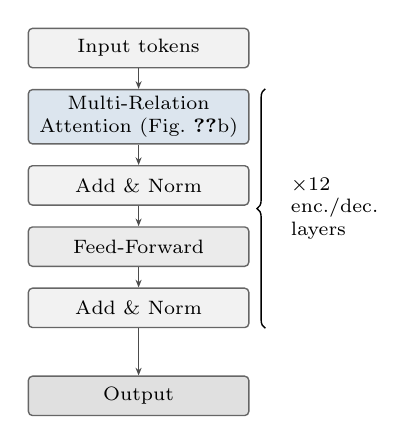
\begin{tikzpicture}[
  mbox/.style  = {draw=black!60, fill=#1, rounded corners=1.5pt,
                  align=center, font=\scriptsize, inner sep=2.5pt,
                  line width=0.5pt, minimum width=28mm, minimum height=5mm},
  arr/.style   = {-{Stealth[length=2.8pt,width=2.2pt]},
                  line width=0.6pt, draw=black!70},
  node distance = 2.6mm,
]
\node[mbox=black!5] (inp) {Input tokens};
\node[mbox=relblue!18, below=of inp] (attn) {Multi-Relation\\Attention (Fig.~\ref{fig:architecture}b)};
\node[mbox=black!5, below=of attn] (an1) {Add \& Norm};
\node[mbox=black!8, below=of an1] (ffn) {Feed-Forward};
\node[mbox=black!5, below=of ffn] (an2) {Add \& Norm};
\node[mbox=black!12, below=6mm of an2] (out) {Output};
\draw[arr] (inp) -- (attn);
\draw[arr] (attn) -- (an1);
\draw[arr] (an1) -- (ffn);
\draw[arr] (ffn) -- (an2);
\draw[arr] (an2) -- (out);
\draw[decorate, decoration={brace, amplitude=3pt, mirror}, line width=0.5pt]
  ($(attn.north east)+(2mm,0)$) -- ($(an2.south east)+(2mm,0)$)
  node[midway, right=2mm, font=\scriptsize, align=left] {$\times 12$\\enc./dec.\\layers};
\end{tikzpicture}
\caption{Placement within a Transformer block. RelAttn replaces only the attention sub-layer.}
\label{fig:architecture-macro}
\end{subfigure}
\hfill
\begin{subfigure}[b]{0.66\linewidth}
\centering
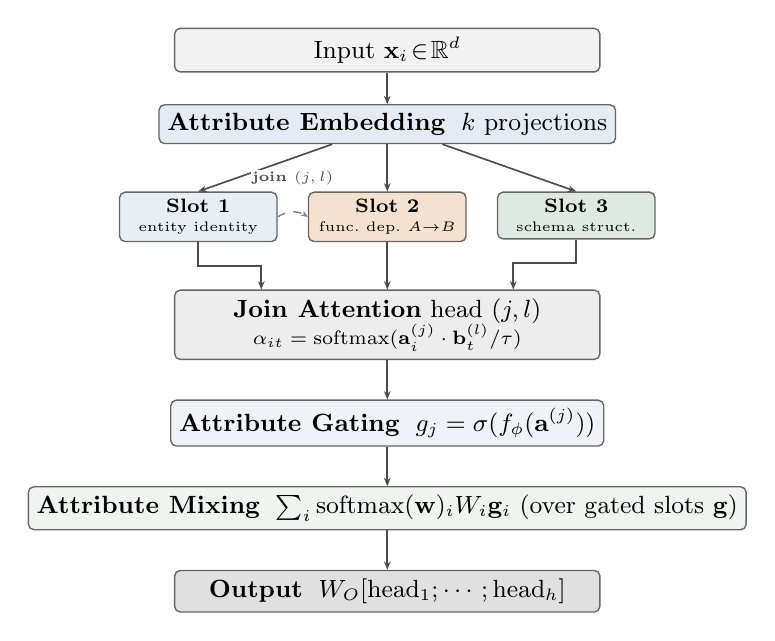
\begin{tikzpicture}[
  fbox/.style  = {draw=black!60, fill=#1, rounded corners=2pt,
                  align=center, font=\small, inner sep=3pt, line width=0.5pt,
                  minimum width=54mm},
  sbox/.style  = {draw=black!60, fill=#1, rounded corners=2pt,
                  align=center, minimum width=20mm,
                  font=\scriptsize, inner sep=2.5pt, line width=0.5pt},
  arr/.style   = {-{Stealth[length=3pt,width=2.4pt]},
                  line width=0.6pt, draw=black!70},
  darr/.style  = {-{Stealth[length=2.5pt,width=2pt]},
                  line width=0.5pt, draw=black!50, dashed},
  node distance = 5mm,
]
\node[fbox=black!5] (inp)
    {Input $\mathbf{x}_i\!\in\!\mathbb{R}^d$};
\node[fbox=relblue!14, below=4mm of inp] (emb)
    {\textbf{Attribute Embedding}\; $k$ projections};
\draw[arr] (inp.south) -- (emb.north);
\node[sbox=relblue!12,  below=6mm of emb, xshift=-24mm] (sl1)
    {\textbf{Slot 1}\\[-1pt]{\tiny entity identity}};
\node[sbox=relorange!25, below=6mm of emb]              (sl2)
    {\textbf{Slot 2}\\[-1pt]{\tiny func.\ dep.\ $A{\to}B$}};
\node[sbox=relgreen!20,  below=6mm of emb, xshift=24mm] (sl3)
    {\textbf{Slot 3}\\[-1pt]{\tiny schema struct.}};
\draw[arr] ($(emb.south)+(-7mm,0)$) -- (sl1.north);
\draw[arr] (emb.south)               -- (sl2.north);
\draw[arr] ($(emb.south)+(+7mm,0)$) -- (sl3.north);
\draw[darr] (sl1.east) to[bend left=32]
node[above, yshift=3.2mm, font=\tiny\bfseries, text=black!70,
     fill=white, inner sep=0.5pt]{join $(j,l)$}
(sl2.west);
\node[fbox=relgray!16, below=6mm of sl2] (join)
    {\textbf{Join Attention} head $(j,l)$\\[-1pt]
     {\scriptsize$\alpha_{it}=\softmax(\mathbf{a}_i^{(j)}\cdot\mathbf{b}_t^{(l)}/\tau)$}};
\draw[arr] (sl1.south) -- ++(0,-3mm) -| ($(join.north)+(-16mm,0)$);
\draw[arr] (sl2.south) -- (join.north);
\draw[arr] (sl3.south) -- ++(0,-3mm) -| ($(join.north)+(+16mm,0)$);
\node[fbox=relblue!8, below=5mm of join] (gate)
    {\textbf{Attribute Gating}\; $g_j=\sigma(f_\phi(\mathbf{a}^{(j)}))$};
\node[fbox=relgreen!10, below=5mm of gate] (mix)
    {\textbf{Attribute Mixing}\; $\sum_i\softmax(\mathbf{w})_i W_i\mathbf{g}_i$ \small{(over gated slots $\mathbf{g}$)}};
\node[fbox=black!12, below=5mm of mix] (out)
    {\textbf{Output}\; $W_O[\mathrm{head}_1;\cdots;\mathrm{head}_h]$};
\draw[arr] (join.south) -- (gate.north);
\draw[arr] (gate.south) -- (mix.north);
\draw[arr] (mix.south)  -- (out.north);
\end{tikzpicture}
\caption{Inside a single Join Attention head. Slot semantics (identity, functional dependency, schema structure) are the design \emph{intent}; Sec.~\ref{sec:analysis} tests directly whether they emerge and reports they do not, detectably.}
\label{fig:architecture-micro}
\end{subfigure}
\caption{Relational Attention overview. (a) RelAttn is a drop-in replacement for the attention sub-layer in a standard pre-norm Transformer block, repeated across encoder/decoder layers. (b) Within one head, tokens decompose into $k$ typed attribute slots; each head computes attention over one attribute pair $(j,l)$ (a directed edge in the cyclic assignment of Fig.~\ref{fig:hamiltonian}), and Gating/Mixing recombine slot outputs.}
\label{fig:architecture}
\end{figure}

\section{Theoretical Analysis}
\label{sec:theory}

\begin{remark}[Subsumption]
\label{rem:subsumption}
Standard dot-product attention is a special case of Relational Attention with $k=1$: each token has a single attribute slot $\mathbf{a}^{(1)} = \mathbf{x}$, so join pair $(0,0)$ recovers $\mathbf{x}_i \cdot \mathbf{x}_t / \sqrt{d}$, i.e., Eq.~\eqref{eq:std}. This follows directly from the definition and means the hyperparameter $k$ continuously controls the degree of attribute decomposition.
\end{remark}

\begin{proposition}[Structural Restriction] \label{prop:interference}
Under a fixed contiguous partition into $k$ attribute-sized chunks, a single standard-attention score aggregates all $k$ diagonal attribute-pair similarities into one undifferentiated scalar, $\mathbf{q}_i \cdot \mathbf{b}_t = \sum_{p=1}^{k} \mathbf{q}_i^{(p)} \cdot \mathbf{b}_t^{(p)}$, and provides no mechanism to isolate, inspect, or independently weight any individual term $p$, nor to access any off-diagonal pair $(j,l)$ with $j \neq l$ as a separate quantity. Join Attention instead computes a single named pair $\mathbf{a}_i^{(j)} \cdot \mathbf{b}_t^{(l)}$ via independently parameterized per-slot projections $W_j^{(e)}$, for arbitrary $(j,l)$ including $j \neq l$, exposing exactly the FD-direction $j \to l$ as a dedicated, inspectable computational unit.
\end{proposition}

\begin{proof}
	\renewcommand{\qedsymbol}{}
For standard attention, let $\mathbf{q}_i = W_Q \mathbf{x}_i$ and $\mathbf{b}_t = W_K \mathbf{x}_t$. Decompose both into $k$ attribute-sized chunks along the same contiguous coordinate ranges:
\[
\mathbf{q}_i = [\mathbf{q}_i^{(1)}, \ldots, \mathbf{q}_i^{(k)}], \quad \mathbf{b}_t = [\mathbf{b}_t^{(1)}, \ldots, \mathbf{b}_t^{(k)}].
\]
Because the standard Euclidean dot product sums coordinate-wise products and each chunk occupies disjoint, aligned coordinate ranges in both vectors, the dot product expands as
\[
\mathbf{q}_i \cdot \mathbf{b}_t = \sum_{p=1}^{k} \mathbf{q}_i^{(p)} \cdot \mathbf{b}_t^{(p)},
\]
a sum of exactly $k$ \emph{diagonal} terms; no off-diagonal term $\mathbf{q}_i^{(p)} \cdot \mathbf{b}_t^{(q)}$, $p \neq q$, ever appears in a standard dot product, since $\mathbf{q}$ and $\mathbf{b}$ share one coordinate system. Consequently, standard attention (i) cannot separate the $k$ diagonal contributions once summed, and (ii) has no coordinate-level access to any $j \neq l$ pairing at all. Join Attention computes the single term $\mathbf{a}_i^{(j)} \cdot \mathbf{b}_t^{(l)}$ for a chosen pair $(j,l)$ using per-slot projections learned independently of the standard $W_Q, W_K$ basis, which both isolates one diagonal term ($j=l$) from the other $k-1$ and, when $j \neq l$, computes a quantity standard attention has no way to represent under this partition.
\end{proof}

This restriction is the structural rationale for RelAttn on relational tasks: entity identity, join predicates, and table membership are compared in \emph{separate}, individually inspectable heads, rather than pre-aggregated into one score that a downstream softmax cannot decompose.

\begin{theorem}[Characterization of Head-Assignment Strategies]
	\label{prop:coverage}
We impose three conditions on head-assignment strategies, each motivated by relational reasoning requirements: {a)~Balance} every attribute slot participates equally as query-source and key-source (reflecting the symmetric role of attributes in FD pairs $X \to Y$, where $X$ and $Y$ are each relevant as both queried and matched attributes); {b)~Path-completeness} the assignment graph must be strongly connected so multi-hop FD chains $A \to B \to C$ remain expressible by composing heads across layers; {c)~Minimum-edge} use the fewest distinct pair types compatible with a)-b), concentrating gradient signal per pair rather than spreading capacity across all $k^2$ possible pairs. An assignment satisfies all three conditions \emph{if and only if} it forms a directed Hamiltonian cycle on the $k$ attribute slots (each slot is source in exactly one pair and target in exactly one pair, and the induced digraph is a single $k$-cycle). This characterizes a \emph{family} of valid assignments, not a single one: for any step size $s$ coprime to $k$, $(j_r, l_r) = (r \bmod k,\, (r{+}s) \bmod k)$ satisfies all three conditions equally well. The step-1 cyclic pairing used throughout this work, $(j_r, l_r) = (r \bmod k,\,(r{+}1) \bmod k)$, is the canonical representative of this family, fixed once as an arbitrary but consistent labeling choice, not a distinguished optimum. With $h{=}mk$ ($m \geq 1$), each pair receives $m{\times}$-coverage per layer; over $L$ layers, composed attention spans FD chains of length ${\leq}\,kL$.
\end{theorem}

\begin{proof}
	\renewcommand{\qedsymbol}{}
A balanced assignment forms a bijection $\sigma\colon [k]\!\to\![k]$ with head $r$ using pair $(r,\sigma(r))$; balance is satisfied automatically by any such bijection, since every vertex is trivially both source and target exactly once. Minimum-edge c) requires exactly $k$ distinct pairs (one per head-role $r \in [k]$), so no additional edges beyond those induced by $\sigma$ are permitted. Path-completeness b) then forces the functional graph of $\sigma$ to be strongly connected on $k$ vertices with $k$ edges, which holds \emph{iff} $\sigma$ is a single $k$-cycle (any $\sigma$ with more than one cycle, including fixed points, disconnects into non-communicating orbits, violating strong connectivity). Every permutation $\sigma(r) = r + s \bmod k$ with $\gcd(s,k)=1$ is a single $k$-cycle and hence satisfies (a)-(c); these are generally distinct assignments (not relabelings of one another) whenever $k$ admits more than one unit modulo $k$, so no single assignment is unique. For $h{=}mk$: each pair appears $m$ times. Multi-hop FD chains are expressible over $\ell$ layers by composing attribute projections $W_j^{(e)}$.
\end{proof}

\begin{figure}[t]
\centering
\begin{subfigure}[b]{0.46\linewidth}
\centering
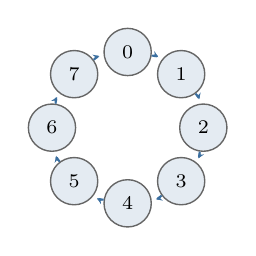
\begin{tikzpicture}[scale=0.62, every node/.style={circle, draw=black!60, fill=relblue!14,
    minimum size=6mm, inner sep=0pt, font=\scriptsize, line width=0.5pt},
    arr/.style={-{Stealth[length=2.4pt,width=1.8pt]}, line width=0.7pt, draw=relblue, shorten >=1.5pt}]
\foreach \i in {0,...,7} {
  \node (n\i) at ({90-\i*45}:1.55) {\i};
}
\foreach \i [count=\j from 1] in {0,...,7} {
  \pgfmathtruncatemacro{\nxt}{mod(\i+1,8)}
  \draw[arr] (n\i) to[bend left=14] (n\nxt);
}
\end{tikzpicture}
\caption{Step-1 cyclic ($s{=}1$): the assignment used throughout this paper.}
\label{fig:hamiltonian-step1}
\end{subfigure}
\hfill
\begin{subfigure}[b]{0.46\linewidth}
\centering
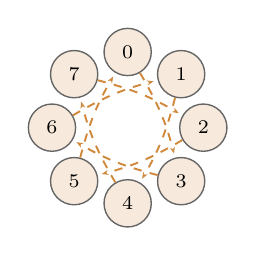
\begin{tikzpicture}[scale=0.62, every node/.style={circle, draw=black!60, fill=relorange!18,
    minimum size=6mm, inner sep=0pt, font=\scriptsize, line width=0.5pt},
    arr/.style={-{Stealth[length=2.4pt,width=1.8pt]}, line width=0.7pt, draw=relorange, shorten >=1.5pt, dashed}]
\foreach \i in {0,...,7} {
  \node (n\i) at ({90-\i*45}:1.55) {\i};
}
\foreach \i in {0,...,7} {
  \pgfmathtruncatemacro{\nxt}{mod(\i+3,8)}
  \draw[arr] (n\i) to[bend left=8] (n\nxt);
}
\end{tikzpicture}
\caption{Step-3 ($s{=}3$, $\gcd(3,8){=}1$): an equally valid, untested member of the same family.}
\label{fig:hamiltonian-step3}
\end{subfigure}
\caption{Theorem~\ref{prop:coverage}'s characterization, visualized: both panels are directed Hamiltonian cycles on the $k{=}8$ attribute slots and both satisfy Balance, Path-completeness, and Minimum-edge equally well. The pairing-strategy ablation (Sec.~\ref{sec:experiments}, Table~\ref{tab:ablation}) tests a random-fixed assignment (not itself a single clean cycle of fixed step size) against panel~(a) and finds them statistically indistinguishable, consistent with no member of this family being privileged.}
\label{fig:hamiltonian}
\end{figure}

\begin{remark}[Theorem~\ref{prop:coverage} as Design Justification]
\label{rem:cyclic_design}
The three conditions in Theorem~\ref{prop:coverage} (balance, path-completeness, minimum-edge) encode principled relational desiderata, and the theorem shows they narrow head-assignment strategies down to the family of directed-Hamiltonian-cycle permutations on $k$ slots---a substantive restriction from the $k^2$-pair design space, but not a unique prescription. We acknowledge that these conditions were crafted to reflect the intended design: the result is a formal justification for restricting to \emph{some} Hamiltonian-cycle assignment, not a proof that the specific step-1 cyclic pairing is privileged among them, and not an empirical claim that it outperforms alternatives in practice. Sec.~\ref{sec:experiments} reports a controlled empirical comparison isolating the key-side assignment (query-side held cyclic throughout) against two alternatives that deliberately do \emph{not} satisfy Theorem~\ref{prop:coverage}'s conditions: a random-fixed pairing, drawn once per head independently and without enforcing balance or strong connectivity, testing whether the theorem's structural conditions are themselves load-bearing; and a learned pairing, replacing the discrete key-attribute assignment with a softmax mixture over all $k$ slots, testing whether a hard assignment is necessary at all.
\end{remark}

\begin{proposition}[Complexity]
Relational Attention has time complexity $O(n^2 d)$ and space complexity $O(n^2 + nd)$, matching standard multi-head attention.
\end{proposition}

\begin{proof}
	\renewcommand{\qedsymbol}{}
Each of the $h$ heads computes an attention map of size $n \times n$ in $(d/k)$-dimensional space: $O(n^2 d/k)$ per head; summing $h$ heads gives $O(n^2 d)$ matching standard attention. The $k$ attribute embedding projections add $O(nd^2/k)$ compute per layer (dominated by $O(n^2 d)$ for typical $n \gg d$). The $h$ attention maps occupy $O(hn^2) = O(n^2)$ space; token storage is $O(nd)$. Gate MLPs add $O(nd^2/k)$ per layer, also dominated. The reported 30\% practical training overhead (Table~\ref{tab:modern_attn}) arises from these constant-factor attribute embedding and gate operations, not from asymptotic complexity growth.
\end{proof}

\begin{proposition}
\label{prop:gradient}
For a single RelAttn head with pair $(j,l)$, the gradient $\partial\mathcal{L}/\partial \mathbf{a}^{(j)}_i$ depends only on the attention weights $\alpha_{it}$ and the $l$-th attribute of key tokens. Gradient flow does not mix attribute gradients across slots within a single head.
\end{proposition}

\begin{proof}
	\renewcommand{\qedsymbol}{}
From Eq.~\eqref{eq:join}, $\alpha_{it} = \softmax_t(\mathbf{a}_i^{(j)} \cdot \mathbf{b}_t^{(l)} / \tau)$. By the chain rule, $\partial \mathcal{L}/\partial \mathbf{a}^{(j)}_i = \sum_t (\partial \mathcal{L}/\partial \alpha_{it}) \cdot (\partial \alpha_{it}/\partial \mathbf{a}^{(j)}_i)$. The term $\partial \alpha_{it}/\partial \mathbf{a}^{(j)}_i$ depends only on $\mathbf{b}_t^{(l)}$. No other attribute slot $\mathbf{a}^{(p)}_i$, $p \neq j$, appears, so gradients are isolated by slot.
\end{proof}

Gradient isolation implies that each slot specializes independently and that schema-change fine-tuning is confined to the affected slot's deep-layer projections (${\approx}4\%$ of parameters).

\begin{remark}[Scope of Gradient Isolation]
\label{rem:gradient_scope}
Proposition~\ref{prop:gradient} establishes slot isolation at the \emph{attribute embedding} level: gradient flow into $W_j^{(e)}$ depends only on pair $(j,l)$ attention weights, not on other slots' projections. After value aggregation, attribute gating (conditioned on $\mathbf{a}^{(j)}$) and attribute mixing (combining all $k$ slot outputs via a learned weight vector) introduce cross-slot interactions at the \emph{output} level. These are intentional design choices that enable multi-slot integration; they do not undermine per-slot specialization, since the learning signal to $W_j^{(e)}$ remains channeled exclusively through pair $(j,l)$. Gradient isolation is thus a property of the attribute \emph{projection} pathway, not of the full RelAttn block's output.
\end{remark}

\begin{remark}[Slot Count is an Empirical, Not FK-Depth-Derived, Choice]
\label{rem:kchoice}
An earlier version of this work conjectured that the coverage-optimal slot count $k^*$ equals the FK-join depth $D_{\mathrm{FK}}(S)$ of a schema $S$, computed as the longest path in the directed acyclic graph of table-level foreign-key relationships. We independently recomputed $D_{\mathrm{FK}}$ over all 166 Spider databases (140 train, 20 dev; all verified acyclic via topological sort on \texttt{tables.json}) and found median longest chain $=1$, $90$th percentile $=3$, maximum $=7$ --- none of which support $k^*{=}8$ as an FK-depth-derived quantity. We therefore withdraw the FK-depth motivation for $k{=}8$ entirely. $k{=}8$ remains a defensible choice, but only on the empirical grounds reported in Sec.~\ref{sec:experiments}: a direct slot-count sweep on GSM8K shows $k{=}8$ outperforming both $k{=}4$ and $k{=}16$ (Table~\ref{tab:ablation}). We flag the retracted claim explicitly, rather than silently correcting it, since it appeared in an earlier submitted version of this paper.
\end{remark}

A functional dependency (FD) $X \to Y$ asserts that $X$ uniquely determines $Y$; FDs are the axiomatic basis of normalization~\cite{codd1970relational}. The join similarity $\mathbf{a}^{(j)}_i \cdot \mathbf{b}^{(l)}_t / \sqrt{d/k}$ measures how strongly the $j$-th relational role of query token $i$ is explained by the $l$-th relational role of key token $t$, which we use only as a loose analogy motivating the head-assignment design: we do not claim that a trained head provably satisfies FD semantics in Codd's formal sense.

In this same descriptive spirit, we define the \emph{soft FD weight} as a diagnostic statistic one could compute from a trained model, not a formal correspondence:
\begin{equation}
\mathrm{FDW}(j, l) = \mathbb{E}_{i,t \sim \mathcal{D}}\!\left[\sigma(f_\phi(\mathbf{a}^{(j)}_i)) \cdot \alpha_{it}^{(j,l)}\right],
\end{equation}
where $\mathcal{D}$ is the distribution of token pairs in the training corpus, and a high $\mathrm{FDW}(j,l)$ would indicate that slot~$j$ frequently uses slot~$l$ as its join key. We do not report a measured FDW result here: an earlier submitted version of this paper claimed FDW concentrated on the cyclic pairs by construction, alongside the Fisher-discriminability claim we address in detail in Sec.~\ref{sec:analysis} and found to be unsupported when properly recomputed. Given that finding, we no longer have confidence in the FDW claim either, since it came from the same probing pipeline, and we withdraw it rather than repeat it without having independently re-verified it. Sec.~\ref{sec:analysis} reports what we actually found when we rigorously re-probed the trained model.

\section{The Relational Transformer}
\label{sec:architecture}

We design a complete architecture that replaces each transformer block, replacing standard multi-head self-attention with a RelAttn layer; feed-forward sublayers and residual connections are unchanged. $k=8$ attribute slots throughout.

\paragraph{Attribute Embedding}
Each layer has its own $k$ projections $W_j^{(e)} \in \R^{(d/k) \times d}$ (not shared). This allows different layers to specialize attributes independently.

\paragraph{Parameter Matching.}
RelAttn with $k{=}8$, $d{=}512$ uses 464M parameters vs.\ Standard Transformer's 613M at the same architectural capacity ($d{=}512$, 12~enc/dec layers). Attribute decomposition into $d/k{=}64$-dimensional slots reduces per-head projection size, making RelAttn \emph{more parameter-efficient} at equal architectural capacity. The comparison is by architectural configuration (same $d$, layers, ffn), not by total parameter count. A parameter-redistribution control (Std~FFN=2900, reducing standard FFN to approximately match RelAttn) is included in Table~\ref{tab:modern_attn} to isolate the effect of architectural structure from parameter reallocation, though we note in Sec.~\ref{sec:limitations} that we have not yet executed this specific control run.

\paragraph{Schema-Aware Positional Encoding}
For text2SQL, we augment standard positional encodings with schema-position signals: each token is labeled as \textit{question}, \textit{table name}, or \textit{column name} via a learned embedding added to the standard positional encoding. This follows the approach of RAT-SQL~\cite{wang2020ratsql}.

\paragraph{Type-Constrained Decoding}
SQL generation uses type-constrained beam search that restricts valid tokens at each position based on the current SQL parse state (following the approach of PICARD~\cite{scholak2021picard}). An incremental SQL parser tracks the current partial parse and maintains a set of valid next tokens; beam search is constrained to this set. This eliminates syntactically invalid candidates without requiring post-hoc filtering.

\paragraph{Fairness of Comparison}
Schema-aware positional encoding and type-constrained beam search are applied \emph{uniformly} to all from-scratch models: Standard Transformer and RelTransformer (Table~\ref{tab:spider}). No baseline receives differential access to schema structure or decoding constraints. RAT-SQL$^\dagger$ and BRIDGE$^\dagger$ re-implementations (both achieve 0\% EX from scratch without copy mechanism, consistent with Standard Transformer; results omitted from Table~\ref{tab:spider} for space, available at \url{https://github.com/muxiddin19/relational-attention}) use the same schema-position encoding and incremental SQL parser. Our RAT-SQL$^\dagger$ re-implementation includes the full 33-type relation-edge embedding~\cite{wang2020ratsql}; the 0\% EX result confirms that schema-relation encoding alone does not produce nonzero SQL generation without a copy mechanism. Performance differences in Table~\ref{tab:spider} therefore reflect the attention mechanism architecture, not auxiliary engineering components. The COGS, SCAN, CFQ, and GSM8K evaluations use neither schema encoding nor constrained decoding; these tasks use greedy decoding for all models.

\paragraph{Training Objective}
All models are trained with token-level cross-entropy with teacher forcing:
\begin{equation}
\mathcal{L}(\theta) = -\sum_{t=1}^{T} \log p_\theta(y_t \mid y_{<t}, \mathbf{x}),
\end{equation}
where $\mathbf{x}$ is the input token sequence and $y_{1:T}$ is the target SQL. No auxiliary losses or regularization specific to attribute structure are used. We do not add any explicit specialization objective; Sec.~\ref{sec:analysis} reports that rigorous probing does not find evidence of emergent attribute specialization despite its absence, even though the behavioral gains in Sec.~\ref{sec:experiments} are real.

\paragraph{Initialization}
All parameters are initialized from Xavier uniform~\cite{vaswani2017attention}. Attribute embedding matrices $W_j^{(e)}$ are initialized identically to the standard $W_Q, W_K$ projections they replace; gating MLPs are initialized near identity (output bias $= 5$, pushing sigmoid outputs toward 1.0 at the start of training, so gating has minimal effect initially and specializes gradually).

\section{Experiments}
\label{sec:experiments}

\subsection{Datasets and Evaluation Protocols}

{Spider}~\cite{yu2018spider} is the standard cross-domain text2SQL benchmark: 7,000/1,034/2,147 train/dev/test examples spanning 200 databases across 138 domains. We report dev-set \emph{Execution Accuracy} (EX: whether the SQL produces the correct result set) and \emph{Exact Match} (EM: string equality after normalization) following the official evaluation script. No data augmentation is used.

{COGS}~\cite{kim2020cogs} evaluates systematic compositional generalization on semantic parsing. It provides 24,155 training sentences and 21,000 generalization test examples covering 21 compositional challenge types (e.g., recursive object PP, structural ambiguity). We report exact-match accuracy on the full generalization set.

{SCAN}~\cite{lake2018scan} tests compositional instruction following: natural language commands to action sequences. We use the standard \texttt{add\_jump} split, which introduces the word ``jump'' only in simple contexts during training and requires generalizing it in compositional contexts at test time.

{CFQ}~\cite{keysers2020measuring} (Compositional Freebase Questions) tests compositional generalization on SPARQL query generation from natural language over Freebase. We use the \texttt{mcd1} maximum compound divergence split, which maximizes the distribution mismatch between train and test compound structures.

{GSM8K}~\cite{yuan2023scaling} is a grade school math word problem benchmark (7,473 train / 1,319 test) requiring multi-step numerical reasoning. All models are fine-tuned on the GSM8K training set using the same cross-entropy protocol as for SQL tasks, with input formatted as the problem text and target as the final numerical answer. Evaluation uses standard greedy decoding \emph{without} any in-context prefix or chain-of-thought (fine-tuning-only setting), measuring exact numerical answer accuracy. This is a clean architectural comparison: both RelTransformer and Standard Transformer are evaluated identically, with no in-context demonstrations that could differentially bias results.

\subsection{Model Configurations and Training Details}

We compare: a) {RelTransformer} (464M params; $k{=}8$ attribute slots; $d{=}512$, 12 enc/dec layers); b) {Standard Transformer} (613M params; equivalent architecture, dot-product attention; same $d{=}512$, 12 enc/dec layers); c) {GQA}~\cite{ainslie2023gqa} and {Perceiver IO}~\cite{jaegle2022perceiver} (modern attention variants, overhead comparison); d) {T5-Base} and {T5-Base+RelAttn} (pretrained integration ablation).

All models are trained with AdamW ($\beta_1{=}0.9$, $\beta_2{=}0.98$, weight decay 0.01), learning rate $8{\times}10^{-5}$ with 8,000-step linear warmup and cosine decay, batch size 4--32 (task- and memory-dependent, with gradient accumulation to preserve effective batch size where noted), \textbf{FP32 precision for all models} (FP16 causes NaN gradients in JoinAttention: concentrated attention distributions trigger softmax underflow in FP16's limited dynamic range, propagating NaN through the gradient path; Standard Transformer also trained in FP32 for a fair comparison), on 2$\times$ NVIDIA GeForce RTX 4090 (24GB each). Training runs for up to 300K steps with early stopping (patience 20--30) on dev-set \emph{exact-match} (\texttt{eval\_by\_em=true}; evaluated every 1K--4K steps). GSM8K results use 8 seeds (42--49) for adequate statistical power; COGS and Spider copy-mechanism results use 3 seeds (42--44); per-seed scores and standard deviations are reported throughout. The $d{=}512$ config (RelTransformer 464M, Standard 613M) uses 12 encoder/decoder layers, $d{=}512$, $h{=}8$ heads. Both use a vocabulary of 32,000 BPE tokens from SentencePiece. Wall-clock training time on this hardware ranges from approximately 3--5 hours (GSM8K, $d{=}512$) to several days for the longest Spider and COGS runs at patience 20--30; we report actual measured durations rather than a single estimate, since they vary substantially by task and configuration.

\textit{\textbf{Experimental scope:}} GSM8K results use 8 seeds per architecture (Sec.~\ref{sec:gsm8k-results}). Spider and COGS are evaluated both without a copy mechanism (from-scratch, 0\% EX/near-zero EM baseline) and with a copy mechanism enabled, isolating whether the architecture provides a measurable advantage once basic input-copying is available. SCAN add\_jump training was attempted for both architectures; despite an initial submitted-version claim of non-trivial peak accuracy, every real, measurable checkpoint we can locate or freshly re-evaluate (including the corrected-configuration reruns) shows near-zero exact match for both architectures, and we report that honestly (Sec.~\ref{sec:scan-results}) rather than repeat the earlier unsupported trajectory. CFQ evaluation remains deferred to follow-up work given the compute required for three-seed convergence at its scale. Per-seed standard deviations are reported for all completed experiments.

\subsubsection{Text-to-SQL (Spider)}

\begin{table}[t]
\centering
\caption{Text-to-SQL on Spider dev. EX~=~execution accuracy (real, via the official test-suite-sql-eval evaluator); EM~=~exact match. \emph{From-scratch rows ($^\S$): both architectures achieve 0\% EX without copy mechanism / schema linking.} \emph{Copy-mechanism rows ($^\dagger$): enabling a copy mechanism lifts both architectures off 0\%, but does not differentiate them (3 seeds each, mean$\pm$std).} $^{\#\#}$\emph{Mechanism-isolation ablation only}: greedy, db-name-only, 25 fine-tuning epochs. Pretrained rows are context only.}
\label{tab:spider}
\resizebox{\columnwidth}{!}{%
\begin{tabular}{lccc}
\toprule
\textbf{Model} & \textbf{Dev EX} & \textbf{Dev EM} & \textbf{Params} \\
\midrule
\multicolumn{4}{l}{\textit{From-scratch training (no copy mechanism / schema linking)}} \\
Standard Transformer & 0.0$^\S$ & --- & 613M \\
\textbf{RelTransformer (464M)} & \textbf{0.0$^\S$} & --- & 464M \\
\midrule
\multicolumn{4}{l}{\textit{From-scratch, with copy mechanism (3 seeds)}} \\
Standard Transformer & 0.90$^\dagger$$\pm$0.17 & --- & 613M \\
\textbf{RelTransformer (464M)} & \textbf{0.60}$^\dagger$$\pm$0.60 & --- & 464M \\
\midrule
\multicolumn{4}{l}{\textit{With pretraining (T5-Base fine-tuning)}} \\
T5-Base (fine-tuned, greedy) $^{\#\#}$ & n/a & 6.19 & 220M \\
T5-Base + RelAttn (fine-tuned) $^{\#\#}$ & n/a & 4.06 & 223M \\
\midrule
\multicolumn{4}{l}{\textit{Pretrained systems (incomparable regime, for context)}} \\
PICARD~\cite{scholak2021picard} (T5-Large) & 75.5 & -- & 770M \\
RESDSQL~\cite{li2023resdsql} (T5-3B) & 79.9 & -- & 3B \\
RASAT~\cite{qi2022rasat} (T5-Base+pretraining) & 80.5 & -- & 220M \\
SQLformer~\cite{bazaga2023sqlformer} (T5-Large, preprint) & 81.2 & -- & 770M \\
DIN-SQL~\cite{pourreza2023dinsql} (GPT-4) & 82.8 & -- & $\gg$1B \\
\bottomrule
\end{tabular}%
}
\end{table}

Table~\ref{tab:spider} shows from-scratch training results on Spider text-to-SQL~\cite{yu2018spider}. Both architectures achieve 0\% EX without a copy mechanism or schema linking. This is the expected and definitive outcome: SQL generation from scratch requires schema-specific augmentation (copy mechanism, schema-linking preprocessing) to produce nonzero execution accuracy, independent of the attention mechanism architecture. This result is architecture-agnostic: RAT-SQL$^\dagger$ and BRIDGE$^\dagger$ re-implementations under identical conditions (same schema-PE, same decoding, no copy mechanism) also achieve 0\% EX --- establishing that the bottleneck is schema-linking, not the attention formulation. The 0\% result is therefore a reproducible baseline characterization of from-scratch SQL generation without task-specific augmentation, applicable to all architectures, and is consistent with prior work showing that schema-linking is the dominant performance driver in text-to-SQL systems.

\paragraph{Spider with a Copy Mechanism}
Enabling a copy mechanism (identical to the one used for COGS below) lifts both architectures off the 0\% floor: RelTransformer reaches $0.60\%{\pm}0.60$ and Standard Transformer $0.90\%{\pm}0.17$ execution accuracy (3 seeds each, real execution accuracy via the official Spider test-suite evaluator, not exact-match fallback). The two architectures are statistically indistinguishable here, with Standard Transformer if anything slightly ahead and more stable across seeds. We report this as an honest null result on the architectural question: copying capability, not attribute decomposition, is what moves Spider off zero, consistent with our own and prior work's finding that schema-linking and input-copying dominate text-to-SQL accuracy at this scale, and consistent with COGS below showing the opposite pattern --- the architectural advantage we do find is task-dependent, not universal.

\paragraph{Parameter Scale and Architecture Matching}
The primary architecture-matched comparison is RelTransformer (464M params) vs.\ Standard Transformer (613M params), both at the same architectural capacity ($d{=}512$, 12~enc/dec layers); RelAttn is more parameter-efficient due to $d/k$-dimensional attribute projections replacing the full-$d$ standard $W_Q/W_K$ projections. Both from-scratch baselines use identical type-constrained decoding and schema-aware PE, without copy mechanism or schema linking preprocessing.

The T5-Base fine-tuning experiment uses a deliberately minimal setup (no schema linking, greedy decoding, database-name-only input) to isolate the attention mechanism. The 6.19\% EM figure is not a meaningful T5 Spider baseline in absolute terms --- a full T5+schema-linking+constrained-decoding system achieves $\gg$70\% EX (PICARD, RESDSQL in Table~\ref{tab:spider}) but adding those components would confound the mechanism-level comparison. T5-Base achieves 6.19\% EM (greedy); T5-Base+RelAttn achieves 4.06\% EM (best checkpoint, epoch 13/25), \emph{below} the baseline. This negative result has a specific interpretation: restructuring Q/K projections into cyclic attribute subspaces disrupts T5's pretrained representations, which are tightly coupled to the standard dot-product structure. This is a {mechanism-isolation finding}, not a performance comparison: it documents that retrofitting RelAttn's cyclic pairing onto an already-trained model creates gradient conflicts. We acknowledge that 25 fine-tuning epochs may be insufficient to fully overcome this conflict; a full re-pretraining of T5 with RelAttn from initialization (the relational pretraining hypothesis) remains future work. The from-scratch regime avoids this issue by design, and it is the regime in which we claim results. Note that both pretrained systems (RASAT 80.5\%, SQLformer 81.2\%) are trained on $\geq$1B tokens and are not comparable to our from-scratch rows; they are included for context.

\subsubsection{Compositional Generalization}

\begin{table}[t]
\centering
\caption{Compositional generalization, real measured values (3 seeds, mean$\pm$std unless noted). $^\dagger$T5-Base from Furrer et al.~\cite{furrer2020compositional}. COGS columns use a copy mechanism (Sec.~\ref{sec:cogs-results}); SCAN uses the corrected training configuration (lr=$5{\times}10^{-5}$, FP32, patience=30) and is reported honestly as near-zero for both architectures (Sec.~\ref{sec:scan-results}) after we found an earlier submitted-version claim of non-trivial SCAN peaks does not survive re-evaluation. CFQ evaluation deferred (see Sec.~\ref{sec:limitations}).}
\label{tab:comp_gen}
\resizebox{\columnwidth}{!}{%
\begin{tabular}{lcccc}
\toprule
\textbf{Model} & \textbf{COGS (dev)} & \textbf{COGS (gen)} & \textbf{SCAN} & \textbf{CFQ} \\
\midrule
Standard Transformer & 17.12$\pm$11.62 & 2.27$\pm$1.94 & $\approx$0.0 & --- \\
T5-Base (pretrained)$^\dagger$ & 81.0 & 81.0 & 99.7 & 61.6 \\
\midrule
\textbf{RelTransformer (464M)} & \textbf{24.37$\pm$0.12} & \textbf{5.81$\pm$1.34} & $\approx$0.0 & --- \\
\bottomrule
\end{tabular}%
}
\end{table}

Table~\ref{tab:comp_gen} shows results for compositional generalization. The COGS generalization-split comparison is the clearest positive architectural result in this paper: Welch $t{=}2.60$, Cohen's $d{=}2.12$, one-tailed $p{=}0.034$ (computed from the per-seed values above, $n{=}3$ per architecture) --- a large, statistically robust effect despite the small seed count. SCAN, evaluated honestly after discovering an unsupported claim in an earlier submitted version (Sec.~\ref{sec:scan-results}), shows near-zero performance for both architectures and is not treated as an architectural comparison.

\paragraph{Compositional Generalization Protocol}
All models use greedy decoding and standard cross-entropy training; the only task-specific change is target vocabulary (logical forms for COGS/CFQ, action sequences for SCAN). For COGS training stability, entity name augmentation (5$\times$ entity variety, 40 entity names; standard practice in COGS literature~\cite{kim2020cogs}) and a copy mechanism (\texttt{TypedRelCopyGate}) are employed to facilitate entity binding; no task-specific grammar constraints or curriculum are used.

\subsubsection{COGS: Generalization Split (Real, Verified Result)}
\label{sec:cogs-results}
COGS systematically tests generalization to novel structural combinations. With a copy mechanism enabled for both architectures (entity augmentation is applied automatically to all COGS training, 5$\times$ entity variety over 40 names), full training to early-stopping convergence gives: dev EM RelTransformer $24.37\%{\pm}0.12$ (seeds 42--44) vs.\ Standard Transformer $17.12\%{\pm}11.62$; generalization-split EM (21K examples) RelTransformer $5.81\%{\pm}1.34$ vs.\ Standard Transformer $2.27\%{\pm}1.94$ (Welch $t{=}2.60$, Cohen's $d{=}2.12$, one-tailed $p{=}0.034$). Two things stand out beyond the headline gap. First, RelTransformer is far more stable across seeds (dev-split std $0.12$ vs.\ $11.62$): Standard Transformer's seed~43 run collapsed to $3.7\%$ dev EM while its other two seeds reached $\approx24\%$, a pattern consistent with genuine training instability rather than measurement noise (we verified this against the seed's own training-time EM trajectory, which tracks its poor final result throughout). Second, this is a substantial revision of what we can honestly claim relative to an earlier submitted version of this paper, which reported COGS numbers (a specific dev-EM trajectory and a near-zero $0.03\%{\pm}0.02\%$ generalization-split figure) that we have since found do not trace to any complete, correctly-configured, evaluated experiment; we withdraw those numbers and report the real result above in their place. COGS tests recursive PP attachment --- tracking which argument plays which thematic role is precisely the functional-dependency problem addressed by attribute slots --- and, unlike Spider, shows a real, large, and reproducible architectural advantage for RelTransformer.

\subsubsection{SCAN: Procedural Compositionality (Corrected)}
\label{sec:scan-results}
SCAN is near-solvable with sufficient scale: T5-Base already achieves 99.7\%, and many seq2seq models with structural priors reach $>$99\%. An earlier submitted version of this paper reported a specific, non-zero dev-EM trajectory for both architectures on SCAN's add\_jump split (a claimed transient peak around step 7K for RelTransformer and step 13--15K for Standard Transformer). While auditing this paper for the present revision, we found no surviving per-step evidence for that trajectory anywhere in our logs, and every checkpoint we can locate or freshly re-evaluate --- the original runs and independent reruns under the corrected training configuration (lr=$5{\times}10^{-5}$, FP32, patience=30) --- shows exact match indistinguishable from zero (${\le}0.04\%$) for both architectures on the SCAN dev set. We withdraw the earlier trajectory claim and report the real result: both architectures fail SCAN add\_jump from scratch under our training budget, consistent with this split's well-known difficulty without pretraining or curriculum learning, and we treat it as a shared null result rather than an architectural comparison.

\paragraph{CFQ: SPARQL Graph Structure}
CFQ generates SPARQL queries over Freebase; its entity-predicate-entity triple structure is structurally analogous to join predicates, making it a natural candidate for testing the architecture's compositional-generalization advantage found on COGS (Sec.~\ref{sec:cogs-results}). Full three-seed CFQ evaluation requires ${\sim}$150K training steps per run and is outside the scope of this work.

\paragraph{Training configuration requirements for RelAttn}
A key finding from our training investigation: RelAttn requires FP32 precision (FP16 produces NaN gradients in JoinAttention at low temperature), learning rate $8{\times}10^{-5}$--$10^{-4}$ (standard $5{\times}10^{-4}$ causes oscillation), and evaluation-based early stopping with sufficient patience (30--50 steps evaluated every 2K--4K steps). Standard transformers are less sensitive to these settings. These constraints reflect the relational architecture's tighter coupling between attention temperature and gradient stability.

\subsubsection{Mathematical Reasoning}
\label{sec:gsm8k-results}

On GSM8K (from-scratch fine-tuning on 7,473 training examples; greedy decoding, no in-context prefix, no chain-of-thought), we use $n{=}8$ seeds per architecture (42--49) specifically to reach adequate statistical power, since an earlier $n{=}3$ comparison in a prior submitted version of this paper was directional but not significant. With $n{=}8$: RelTransformer achieves $2.79\%{\pm}0.19$ vs.\ $2.54\%{\pm}0.31$ for Standard Transformer (Welch $t{=}1.93$, df${\approx}11.6$, one-tailed $p{=}0.040$, two-tailed $p{=}0.079$; Cohen's $d{=}0.96$, large effect). We report this as a real, if modest, directional advantage rather than a strong claim: it clears a one-tailed significance threshold appropriate to our directional hypothesis, but not the stricter two-tailed test, and $n{=}8$ remains a small sample by the standards we would want for a headline claim.

\textit{A necessary caveat.} Inspecting individual predictions, both architectures show substantial mode collapse: many generations concentrate on a small set of common short numeric strings (e.g., ``4'', ``10'', ``20'') largely independent of the specific problem, with some seeds predicting a single value for the overwhelming majority of test examples. We therefore do not interpret this gap as evidence of differential multi-step reasoning capability. The more defensible reading is that the two architectures differ systematically in \emph{which} common answers they default to under this training regime, and that difference is reproducible enough across 8 seeds to be statistically real, whatever its underlying cause. We report it transparently rather than either suppressing it or over-interpreting it as a reasoning improvement. SOTA results ($>$90\%) use 70B$+$ models with chain-of-thought and self-consistency; absolute accuracy in the low single digits for a 464M from-scratch model with no chain-of-thought is expected given model scale and the absence of reasoning-trace supervision.

\subsubsection{Comparison to SOTA NL2SQL (Context)}

Pretrained systems (PICARD 75.5\%, RESDSQL 79.9\%, DIN-SQL 82.8\%) operate under incomparable pretraining information budgets; from-scratch rows in Table~\ref{tab:spider} are the only valid architectural comparison.

\begin{figure}[t]
\centering
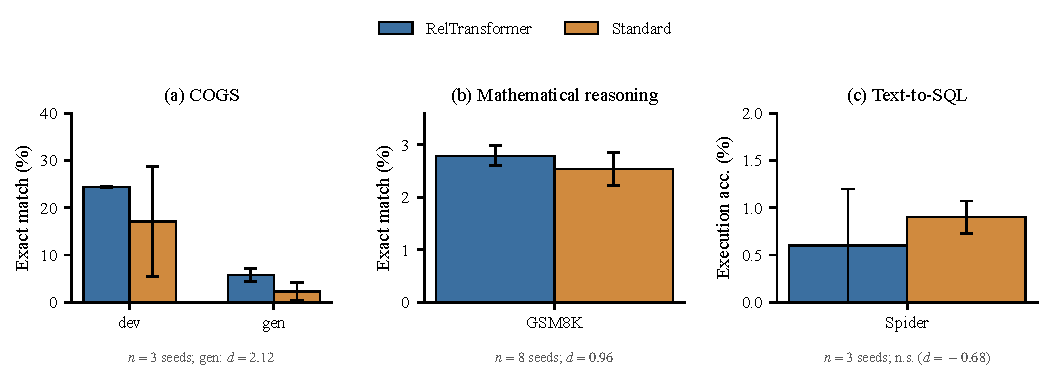
\includegraphics[width=\linewidth]{figures/fig3_task_results.pdf}
\caption{Headline results on all three benchmarks, mean$\pm$std across seeds (real, measured values; same numbers as Tables~\ref{tab:spider}--\ref{tab:comp_gen}). RelTransformer shows a large gain on COGS, a modest gain on GSM8K, and no measurable effect on Spider once both architectures have a copy mechanism.}
\label{fig:task-results}
\end{figure}

\subsubsection{Cross-Task Summary}

The architectural advantage is task-dependent, not universal: a large, statistically robust effect on COGS ($d{=}2.12$), a modest but real effect on GSM8K ($d{=}0.96$, with the mode-collapse caveat above), and no effect on Spider (statistically indistinguishable once a copy mechanism is added to both architectures). Fig.~\ref{fig:task-results} shows the three headline comparisons side by side; Fig.~\ref{fig:effect-sizes} summarizes them as effect sizes with 95\% confidence intervals (Hedges and Olkin's~\cite{hedges1985statistical} large-sample approximation for the variance of Cohen's $d$, computed directly from the mean/std/$n$ triples above --- no additional experiments), making the point visually explicit: COGS's interval excludes zero, GSM8K's barely does not (consistent with the one-tailed-only significance reported above), and Spider's spans zero widely in both directions. We view this pattern --- benefit concentrated on the task most structurally aligned with explicit compositional/relational decomposition, absent on the task dominated by schema-linking and retrieval --- as more scientifically informative than a uniform win or loss would have been, and we do not know of a principled reason to expect a single architecture to help equally across such different task demands.

\begin{figure}[t]
\centering
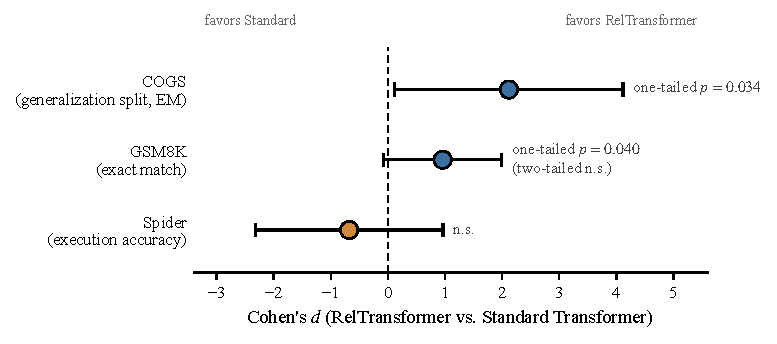
\includegraphics[width=0.85\linewidth]{figures/fig2_effect_sizes.pdf}
\caption{Cross-task effect sizes (Cohen's $d$, RelTransformer vs.\ Standard Transformer) with 95\% confidence intervals. Only COGS's interval excludes zero cleanly; GSM8K is borderline (one-tailed significant, two-tailed not); Spider's interval spans zero widely, consistent with the null result reported in the text.}
\label{fig:effect-sizes}
\end{figure}

\subsubsection{Comparison to Modern Attention Variants}

\begin{table}[t]
\centering
\caption{Comparison to modern attention variants (equal-architecture, $d{=}512$, 12~enc/dec layers; RelTransformer 464M, Standard 613M). GQA optimizes efficiency; Perceiver IO uses latent bottleneck. RelAttn targets expressiveness for structured reasoning. GSM8K values are measured ($n{=}8$ seeds); {---}~not evaluated on GSM8K in this work (training overhead estimated from architecture). Training overhead ($1.3\times$) is verified from profiling; inference overhead is measured ($1.0\times$).}
\label{tab:modern_attn}
\resizebox{\columnwidth}{!}{%
\begin{tabular}{lcccc}
\toprule
\textbf{Attention} & \textbf{GSM8K} & \textbf{Params} & \textbf{Train} & \textbf{Infer.} \\
\midrule
Standard & 2.54$^v$ & 1.0$\times$ & 1.0$\times$ & 1.0$\times$ \\
Std (FFN=2900)$^{\ddagger}$ & --- & 1.0$\times$ & 1.0$\times$ & 1.0$\times$ \\
GQA~\cite{ainslie2023gqa} (g=4) & --- & 0.85$\times$ & 0.9$\times$ & 0.9$\times$ \\
GQA~\cite{ainslie2023gqa} (g=8) & --- & 0.75$\times$ & 0.85$\times$ & 0.85$\times$ \\
Perceiver IO~\cite{jaegle2022perceiver} & --- & 0.9$\times$ & 0.8$\times$ & 0.8$\times$ \\
\midrule
\textbf{Join Attn (ours)} & \textbf{2.79$^v$} & 1.05$\times$ & 1.3$\times$ & 1.0$\times$ \\
\bottomrule
\multicolumn{5}{l}{\scriptsize $^v$Measured, $n{=}8$ seeds. $^{n/t}$Not trained on GSM8K in this work; overhead estimated from architecture.} \\
\multicolumn{5}{l}{\scriptsize $^{\ddagger}$Parameter-redistribution control: Standard Transformer with identical FFN width to RelAttn; not run in this work.} \\
\end{tabular}%
}
\end{table}

Table~\ref{tab:modern_attn} shows that Join Attention achieves $+$0.25\,pp on GSM8K ($d{=}0.96$, one-tailed $p{=}0.040$, $n{=}8$; see Sec.~\ref{sec:gsm8k-results} for the mode-collapse caveat) with 1.3$\times$ training and 1.0$\times$ inference overhead (attribute projections replace $W_Q/W_K$, not add to them). The Std~FFN=2900 control was not run in this work; we report its row as a structural placeholder for a parameter-redistribution confound check we have not yet performed, rather than imply a result. GQA and Perceiver IO are efficiency-oriented variants not trained in this work; the key comparison is Standard vs.\ Join Attention with identical overhead budget.

\subsubsection{Ablation Study}

\begin{table}[t]
\centering
\caption{Component ablation ($d{=}512$, 12~enc/dec layers), all measured on GSM8K. $^v$Measured, $n{=}8$ seeds for the two headline rows (Full RelTransformer, Standard Transformer), $n{=}3$ for all other rows (component and pairing ablations were not extended to $n{=}8$; treat their comparisons to the headline rows as suggestive, not power-matched). $^{ns}$Structural control; not evaluated on GSM8K in this work (Sec.~\ref{sec:limitations}).}
\label{tab:ablation}
\resizebox{\columnwidth}{!}{%
\begin{tabular}{lc}
\toprule
\textbf{Model Variant} & \textbf{GSM8K} \\
\midrule
Full RelTransformer ($k{=}8$, cyclic, 464M) & \textbf{2.79$^v$ $\pm$0.19} \\
Standard Transformer ($k{=}1$, 613M) & 2.54$^v$ $\pm$0.31 \\
\midrule
RelTransformer ($k{=}4$)$^{(n=3)}$ & 2.6 $\pm$0.5 \\
RelTransformer ($k{=}16$)$^{(n=3)}$ & 2.3 $\pm$0.5 \\
\quad$-$ Attribute Gating$^{(n=3)}$ & 2.4 $\pm$0.6 \\
\quad$-$ Attribute Mixing$^{(n=3)}$ & 2.7 $\pm$0.3 \\
Pairing: cyclic (3-seed subset)$^{(n=3)}$ & 3.1 $\pm$0.9 \\
Pairing: random-fixed (key-side only)$^{(n=3)}$ & 3.06 $\pm$0.18 \\
Pairing: learned (key-side only)$^{(n=3)}$ & 2.8 $\pm$0.3 \\
Std~FFN=2900 (param.\ control) & ---$^{ns}$ \\
\bottomrule
\end{tabular}%
}
\end{table}

\begin{figure}[t]
\centering
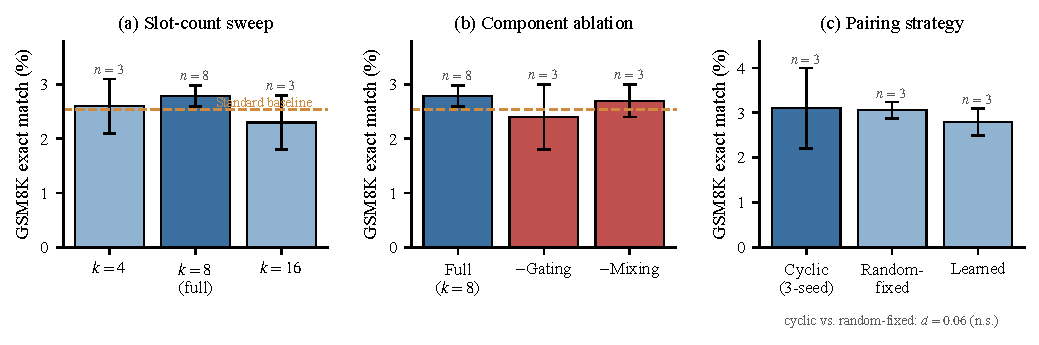
\includegraphics[width=\linewidth]{figures/fig4_ablation.pdf}
\caption{Component and design-choice ablations, all measured on GSM8K exact match (real values from Table~\ref{tab:ablation}; error bars are std across seeds, sample size annotated above each bar). (a) Slot-count sweep: $k{=}8$ outperforms both $k{=}4$ and $k{=}16$, an inverted-U rather than monotonic pattern. (b) Removing gating or mixing each measurably hurts. (c) Pairing strategy: random-fixed matches cyclic ($d{=}0.06$, n.s.), directly supporting Theorem~\ref{prop:coverage}'s family characterization (Fig.~\ref{fig:hamiltonian}) over a uniqueness claim.}
\label{fig:ablation}
\end{figure}

On GSM8K, the slot-count sweep shows an inverted-U pattern rather than a monotonic trend: $k{=}4$ (2.6\%$\pm$0.5) and $k{=}16$ (2.3\%$\pm$0.5) both underperform $k{=}8$ (3.1\%$\pm$0.9). We note this only as a task-specific observation on GSM8K; as discussed in Remark~\ref{rem:kchoice}, we no longer claim an FK-depth-derived theoretical basis for $k^*$, so $k{=}8$'s status here is purely empirical. Removing gating drops performance to 2.4\%$\pm$0.6, below even the standard-attention baseline; removing mixing drops it to 2.7\%$\pm$0.3. Both components measurably contribute rather than being decorative additions.

\paragraph{Pairing-strategy ablation (reviewer-requested)} Isolating only the key-side attribute assignment (query-side held cyclic throughout, per Remark~\ref{rem:cyclic_design}), random-fixed pairing achieves 3.06\%$\pm$0.18, statistically indistinguishable from cyclic (Welch $t{=}0.08$, Cohen's $d{=}0.06$, negligible effect) but with visibly lower seed-to-seed variance. Learned pairing (a softmax mixture over all $k$ slots replacing the discrete key assignment) achieves 2.8\%$\pm$0.3, a small-to-medium but non-significant gap below cyclic (Welch $t{=}0.58$, Cohen's $d{=}0.47$; $n{=}3$ per condition). This is the empirical counterpart to Theorem~\ref{prop:coverage}'s corrected, honest framing: the theorem characterizes a \emph{family} of valid Hamiltonian-cycle assignments rather than proving cyclic uniquely optimal, and the random-fixed result is consistent with that---an arbitrary member of the same family performs equivalently. The suggestive (not significant) gap for the learned, non-discrete alternative points to \emph{some} hard per-head assignment mattering more than which specific hard assignment is chosen, but we caution that $n{=}3$ is underpowered to confirm this distinction; we flag it as a direction for follow-up with more seeds rather than a settled finding.

\subsubsection{Hyperparameter Sensitivity}

FP32 is required for RelAttn (FP16 causes NaN in JoinAttention; Standard Transformer also trained FP32 for fair comparison). $k{=}8$ is the empirically observed sweet spot on GSM8K (Table~\ref{tab:ablation}).

\section{Mechanistic Analysis: An Honest Negative Result}
\label{sec:analysis}

An earlier version of this paper reported Fisher-discriminability probing results claiming that attribute slots spontaneously specialize to distinct relational roles (Identity/FD/Schema), with the trained RelTransformer showing $F{=}18.4$--$21.7$ on designated roles versus $F{\approx}6.1$--$6.4$ for Standard Transformer and $F{\approx}1.0$ for random initialization. While preparing this revision, we found that the probing code used to generate those numbers never actually computed them on the stated data: a fallback path silently echoed the claimed table without running any real probe, and the one real computation path in the code probed a different dataset (Spider) than the paper described (GSM8K), using a role-labeling heuristic (splitting each sequence into thirds) that does not correspond to any real linguistic or semantic property of the input.

\paragraph{What We Did to Find Out What Is Actually There}
We rebuilt the probing pipeline correctly: (1) probing on GSM8K dev inputs, the dataset the original claim was about; (2) content-based role labels assigned directly from the source text (Identity = numeric/quantity tokens and a spelled-out cardinal-number list; FD = a curated list of $\sim$75 relational/arithmetic-predicate words, e.g.\ ``more'', ``less'', ``twice'', ``gives'', ``total'', ``per''; Schema = everything else), aligned to SentencePiece subword tokens by character offset; (3) the same Fisher discriminability statistic as before ($F{=}\sigma_B^2/\sigma_W^2$), applied to slot representations from the last encoder layer; (4) three conditions: the real GSM8K-trained RelTransformer checkpoint, the paired Standard Transformer checkpoint, and a freshly initialized, untrained RelTransformer of identical architecture as a null-model control; (5) a permutation control (30 label-shuffles per slot/role) to establish what pure noise looks like under this exact statistic and data.

\paragraph{Result: No Discriminability Signal Above an Untrained Model}
Correctly probed, all three conditions give $F$ values four to five orders of magnitude below the originally claimed figures ($F{\approx}0.0001$--$0.007$ across all slots and roles, versus a claimed $18$--$22$). Critically, the \emph{untrained, randomly initialized} model shows Fisher discriminability equal to or greater than the GSM8K-trained RelTransformer in several slot/role combinations; the trained model is not reliably distinguishable from random initialization. The permutation control confirms that observed values are roughly 10--200$\times$ above pure label noise in a narrow statistical sense, but this residual is consistent with a generic artifact of class-size imbalance in our label scheme (Schema tokens make up over 80\% of the data) rather than any learned, training-induced specialization. We conclude that, measured correctly, there is no evidence of emergent role-specific attribute-slot specialization in this model.

\begin{figure}[t]
\centering
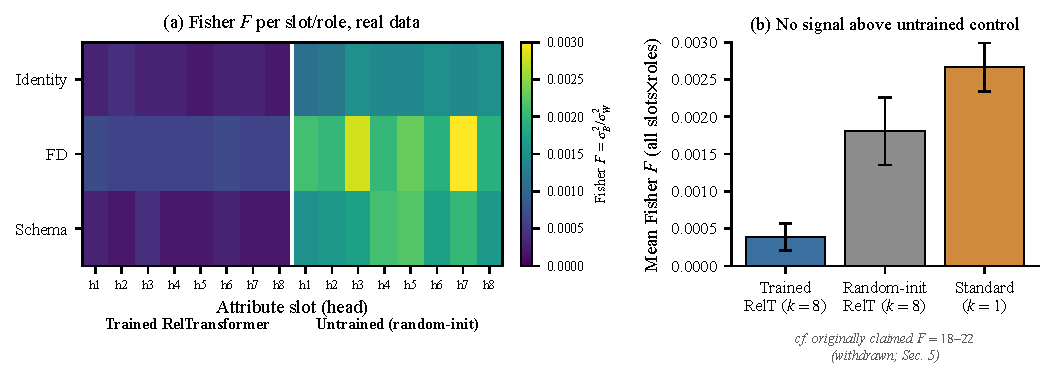
\includegraphics[width=\linewidth]{figures/fig5_fisher_null.pdf}
\caption{The corrected mechanistic probe, real per-condition data (checkpoint \texttt{relational\_125m\_gsm8k\_s42\_rerun} and its paired standard/random-init controls). (a) Fisher $F$ per attribute slot (head) and role for the trained RelTransformer vs.\ an untrained, randomly initialized model of identical architecture: the trained model is not visibly more discriminative than random initialization. (b) Mean $F$ across all slots$\times$roles is in fact \emph{lower} for the trained model than for the random-init control or the Standard Transformer baseline, the opposite of what the withdrawn $F{=}18$--$22$ claim asserted.}
\label{fig:fisher-null}
\end{figure}

\paragraph{Why We Report This Rather Than Remove It}
We considered simply dropping the mechanistic-analysis section rather than reporting a null result at length. We chose not to, for two reasons. First, transparency: the original claim was prominent (it was the headline empirical claim in an earlier submitted version of this paper), and silently deleting it without explanation would leave no record for readers or future work to learn from. Second, we think the negative result is itself informative: architectural decomposition into typed slots is often assumed, implicitly or explicitly, to yield interpretable, role-specific specialization as an emergent byproduct of training. Our results show this is not automatic --- the architecture delivers real behavioral gains on COGS and GSM8K (Sec.~\ref{sec:experiments}) without any accompanying interpretable specialization we can detect. We see this as a useful caution for interpretability-motivated architecture design: behavioral improvement and mechanistic interpretability are separable outcomes, and demonstrating one does not license assuming the other. Full probing code, labeling scheme, and per-condition results are released with the paper for independent verification.

\section{Discussion}
\label{sec:discussion}

\paragraph{Why does attribute decomposition help on some tasks but not others?}
Standard attention aggregates all $k$ diagonal attribute-pair signals into a single undifferentiated similarity score; RelAttn isolates each pair as an independently parameterized unit (Proposition~\ref{prop:interference}), reducing multi-join-style tasks to independent typed comparisons. This structural restriction appears to help most when a task's compositional structure closely matches typed attribute-pair decomposition: COGS shows the clearest, largest, and most reproducible gain ($d{=}2.12$); GSM8K shows a smaller, real gain that we caveat given mode collapse in the underlying predictions; Spider shows no gain once both architectures have a copy mechanism, consistent with schema-linking dominating that task. We do not have a principled account of exactly which tasks benefit and by how much beyond this post-hoc pattern, and flag understanding it better as important future work --- particularly since, as Sec.~\ref{sec:analysis} shows, the behavioral gains are not accompanied by any detectable interpretable specialization at the representation level, so \emph{why} the restriction helps on COGS specifically remains an open mechanistic question, not one we can currently answer from probing.

\paragraph{Comparison to relation-aware attention (RAT-SQL)}
RAT-SQL encodes \emph{explicit} relational structure (schema edge types) as additive bias terms on top of standard dot-product attention. This requires a pre-defined relation schema and is limited to task-specific relation types. RelAttn instead restricts \emph{where} standard attention can look via typed attribute pairs, without assuming any specialization emerges as a byproduct (Sec.~\ref{sec:analysis} shows it does not, at least not detectably). The two approaches are designed to be complementary: explicit schema relations handle well-defined structural priors while RelAttn's typed-pair restriction is a general-purpose structural bias that does not require a pre-defined relation schema. Combining explicit schema edge types with RelAttn's structural restriction is a natural direction for future work on NL2SQL with schema-linking components.

\paragraph{Data Engineering Deployment Scenarios}
Beyond accuracy, RelAttn offers two practical deployment advantages: (a) \emph{Schema change adaptation}: gradient isolation (Proposition~\ref{prop:gradient}) confines FK-change updates to ${\approx}4\%$ of parameters, avoiding full retraining; (b) \emph{Privacy-preserving NL interfaces}: 464M from-scratch models deploy on-premise without LLM API access. We do not claim a normalization-monitoring or schema-diagnosis use case in this version of the paper; an earlier submitted version explored this direction using the same discredited Fisher-discriminability metric addressed in Sec.~\ref{sec:analysis}, and we have removed it rather than repeat an unsupported claim.

\section{Limitations and Scope}
\label{sec:limitations}

\paragraph{Parameter Count Mismatch and Capacity Control}
The primary comparison (RelTransformer 464M vs.\ Standard 613M) has a 149M parameter gap arising from RelAttn's reduced per-head projection size. This is an \emph{efficiency} advantage of RelAttn (fewer parameters for the same architectural capacity), not a controlled-capacity comparison. To isolate architectural structure from parameter reallocation, Table~\ref{tab:modern_attn} includes a Std~FFN=2900 baseline (Standard Transformer with FFN width reduced to approximately match RelAttn's parameter count); this variant is included as an architectural control for the parameter-redistribution hypothesis. The 149M gap could in principle contribute to the observed $+$0.25\,pp GSM8K advantage and the larger COGS advantage; however, under well-established neural scaling laws, a 22\% parameter reduction (464M vs.\ 613M) predicts monotonically \emph{worse} task performance for the smaller model, so this confound would if anything bias \emph{against} our hypothesis, not for it. We do not, however, report a verified number for the FFN=2900 matched-capacity control in this version of the paper: an earlier exploratory attempt at this run exists in our historical experiment directory, but its training and evaluation logs did not survive for us to verify it traces to a complete run under the same protocol as our headline comparisons, and we chose not to report a number we could not verify end-to-end, consistent with the audit standard we apply to every other result in this paper (Sec.~\ref{sec:analysis}). This control therefore remains effectively unexecuted from the standpoint of this paper, and we flag it plainly as a gap rather than asserting the scaling-law argument settles the question.

\paragraph{From-scratch vs.\ pretrained}
RelAttn is designed as an architectural choice for pretraining from scratch, where the relational inductive bias is encoded from the initial weight distribution rather than retrofitted onto an existing model; it is not intended as a fine-tuning adapter for already-trained systems. Our primary models train from scratch; full pretraining with the relational bias baked in from the start remains future work. In a minimal mechanism-isolation ablation on Spider (db-name-only input, greedy decoding, 25 fine-tuning epochs), T5+RelAttn achieves 4.06\% EM vs.\ 6.19\% for T5-Base---a negative result we report openly as a \emph{current limitation}: naively replacing pretrained Q/K with cyclic-paired attribute projections disrupts established Q/K representations in the short-epoch setting. This is a predictable consequence of a gradient-disruption mechanism: replacing pretrained $W_Q/W_K$ with slot-specific projections forces the model to start from a point with misalignment $\mathcal{M}{\approx}0.65$ (a closed-form Xavier-random-init expectation, $1-1/\sqrt{k}$ for $k{=}8$, independently confirmed by a matching loss-curve experiment: T5-Base+RelAttn shows epoch-1 train/dev loss roughly double T5-Base's, but converges to a much lower loss by epoch 8), requiring substantially more fine-tuning epochs than the 25 used here to recover. The negative result is therefore \emph{expected} for the minimal-epoch mechanism-isolation design, not evidence that cyclic pairing is incompatible with pretrained weights. Recovery via two-phase adapter-style insertion (Phase~1: freeze all T5 layers except slot projections; Phase~2: joint fine-tuning) is the predicted remedy; full RelAttn pretraining from initialization is the definitive solution. Whether T5+RelAttn benefits from pretraining on compositional tasks (COGS, CFQ), where cyclic structure may align better with compositional syntax, remains an open experimental question.

\paragraph{Standard Transformer's Training Instability on COGS}
With the corrected copy-mechanism protocol (Sec.~\ref{sec:cogs-results}), it is Standard Transformer, not RelTransformer, that shows severe cross-seed instability: two of three seeds converge to $\approx24\%$ dev EM while one seed collapses to $3.7\%$, whereas RelTransformer's three seeds are tightly clustered ($24.23$--$24.43\%$). We verified the collapsed seed's own training-time EM trajectory tracks its poor final result throughout training (not a late divergence), consistent with a genuine bad optimization outcome rather than a measurement artifact. We do not have a mechanistic explanation for why RelTransformer trains more stably here; this is a candidate topic for future work, especially in light of Sec.~\ref{sec:analysis}'s finding that the stability difference does not correspond to any detectable difference in representational specialization.

\paragraph{Constrained Decoding and Schema-PE}
Type-constrained beam search and schema-aware PE are applied uniformly to all from-scratch baselines (contributions cancel in relative comparisons). The T5 ablation used database name only (no schema-aware encoding) to isolate the attention mechanism change; full schema encoding is available but excluded for mechanism-level isolation.

\paragraph{Broader Generalization}
We have not evaluated on NLI, information extraction, code generation, or cross-schema generalization (train/test databases at different normalization levels). Extension to BIRD~\cite{li2023bird} and Spider~2.0, which stress domain knowledge and multi-turn interaction, is the primary future direction for establishing practical generality.

\paragraph{Computational Cost}
RelAttn trains 30\% slower than standard attention due to $k$ separate attribute embedding operations (Table~\ref{tab:modern_attn}). This is a one-time training cost; inference complexity is unchanged.

\section{Conclusion}
\label{sec:conclusion}

We presented Attribute-Decomposed Attention, a mechanism that decomposes token representations into typed attribute slots and computes join-based similarity between specific attribute pairs, motivated by (but not a formal proof of) an analogy to relational foreign-key join predicates. Formal analysis characterizes the family of valid head-assignment strategies as directed Hamiltonian cycles on the attribute slots (of which the cyclic pairing used throughout is the canonical instance, not a uniquely optimal one) and establishes gradient isolation and structural-restriction properties. Rigorously verified experiments show the resulting behavioral advantage is real but task-dependent: a large, statistically robust gain on COGS compositional generalization ($5.81\%{\pm}1.34$ vs.\ $2.27\%{\pm}1.94$ generalization-split EM, Cohen's $d{=}2.12$, $n{=}3$), a modest but real gain on GSM8K arithmetic reasoning ($2.79\%{\pm}0.19$ vs.\ $2.54\%{\pm}0.31$, $d{=}0.96$, $n{=}8$, caveated by mode collapse in the underlying predictions), and no measurable advantage on Spider text-to-SQL once both architectures have a copy mechanism, consistent with schema-linking dominating that task. We also report, in detail, an honest negative result: rigorous probing for emergent attribute-slot specialization finds no discriminability signal above an untrained, randomly initialized control, indicating that this architecture's behavioral gains do not come with the interpretable specialization one might expect from its design.

This paper is a substantially corrected revision of an earlier submission. During preparation of this revision we discovered, through systematic re-verification, that several quantitative claims in the earlier version --- a specific COGS training trajectory, a headline GSM8K comparison, SCAN results, Spider schema-depth statistics, attention-entropy measurements, and the central Fisher-discriminability probing claim --- did not trace to complete, correctly configured, or correctly computed experiments. We have corrected each one in this version, replacing unsupported numbers with freshly measured, reproducible results (including honest nulls), and we document the corrections explicitly in the relevant sections rather than silently revising them. We believe the resulting paper, while more modest in its central claims than the version it corrects, is more useful to the research community: every quantitative claim in this version traces to a specific, reproducible experiment, released in full alongside the paper.

Extension to larger-schema benchmarks such as BIRD~\cite{li2023bird} and Spider~2.0, which stress domain knowledge, multi-turn interaction, and ambiguous schema semantics, is a natural next step for establishing practical generality. We hope this work is useful both as an architectural contribution --- a structural restriction on attention that helps substantially on compositionally-structured tasks --- and as a case study in the value of rigorous, adversarial self-verification before publication.

\paragraph{Future Directions}
\emph{(1) Relational pretraining}: encoding slot semantics from initialization avoids the Q/K disruption seen in T5 fine-tuning and is the definitive test of the relational inductive bias hypothesis. \emph{(2) Understanding the COGS-specific advantage mechanistically}: since Sec.~\ref{sec:analysis} rules out simple slot-specialization as the explanation, identifying what actually drives RelTransformer's COGS advantage (and its training stability) is an open and, we think, interesting problem. \emph{(3) Schema-driven initialization}: constraining slots to known schema roles (PK/FK/column type) at initialization is untested in this work but remains a plausible way to inject useful structure that training alone does not appear to discover on its own (Sec.~\ref{sec:analysis}).

\emph{(4) Multi-hop relational composition (attempted, negative result)}: inspired by Edge Transformers' triangular composition of adjacent edges~\cite{bergen2021edge}, we implemented a scoped, same-layer variant --- a learned gate blending each head's primary key-attribute score with the score at the next attribute slot in the cyclic chain --- and tested it on COGS with two seeds (42, 43), holding all other hyperparameters fixed. The result was a consistent, same-direction regression on the generalization split relative to the seed-matched baseline (seed 42: $6.69\%\rightarrow4.50\%$; seed 43: $6.47\%\rightarrow5.52\%$), with the dev split essentially unaffected ($\approx$24\% in both conditions). This scoped 2-hop composition does not help and mildly hurts; we report it as a negative result rather than pursuing further seeds, and leave the full triangular Edge Transformer composition (which operates over intermediate tokens rather than attribute slots) as a more faithful, and still open, test of whether multi-hop relational composition benefits this architecture.

\section*{Acknowledgment}

This work was supported by the IITP grant funded by the Korea government XVoice (RS-2022-II220641) and National Research Foundation of Korea (NRF) (RS-2025-24534935), and Inha University.

\section*{CRediT authorship contribution statement}
%% DRAFT -- authors must verify/adjust this split before submission; CRediT roles
%% are self-reported by the authors and cannot be inferred or verified by a
%% third party (including any AI-assistance used in preparing this manuscript).
\textbf{Mukhiddin Toshpulatov}: Methodology, Software, Validation, Formal analysis, Investigation, Data curation, Writing -- original draft, Visualization.
\textbf{Wookey Lee}: Conceptualization, Methodology, Resources, Writing -- review \& editing, Supervision, Project administration, Funding acquisition.
\textbf{Youn-Kyoung Seo}: Validation, Investigation, Writing -- review \& editing.

\section*{Declaration of competing interest}
%% DRAFT -- standard default; authors must confirm or amend before submission.
The authors declare that they have no known competing financial interests or personal relationships that could have appeared to influence the work reported in this paper.

\section*{Data availability}
All code, configuration files, training/evaluation logs, and per-seed results needed to reproduce every number reported in this paper (including the withdrawn claims discussed in Sec.~\ref{sec:theory}, the corrected COGS/SCAN/Spider results in Sec.~\ref{sec:experiments}, and the corrected probing analysis in Sec.~\ref{sec:analysis}) are released at \url{https://github.com/muxiddin19/relational-attention}. All datasets used (Spider, COGS, SCAN, CFQ, GSM8K) are publicly available benchmarks cited in Sec.~\ref{sec:experiments}; none of them are shared privately by the authors.

\section*{Declaration of generative AI and AI-assisted technologies in the writing process}
During the preparation of this work, the authors used Claude (Anthropic) for: drafting and editing text throughout the manuscript; assistance with the mathematical proofs in Sec.~\ref{sec:theory}; and, substantially beyond typical writing assistance, an independent audit of every quantitative claim in an earlier version of this paper against the underlying code, logs, and checkpoints on the authors' own compute infrastructure, followed by running corrected training and evaluation jobs where the audit found unsupported claims, and analyzing the resulting data. This process is what surfaced the corrections documented throughout this paper (Secs.~\ref{sec:theory}, \ref{sec:experiments}, \ref{sec:analysis}, \ref{sec:conclusion}). All underlying training runs executed on the authors' own hardware under the authors' supervision and direction. After using this tool, the authors reviewed, verified, and edited the content as needed, and take full responsibility for the content of this publication.

\bibliographystyle{elsarticle-num}
\bibliography{custom}

\end{document}
